% Copyright (C) 2014-2016 by Thomas Auzinger <thomas@auzinger.name>

\documentclass[draft,final]{vutinfth} % Remove option 'final' to obtain debug information.

\usepackage{listings}
% Load packages to allow in- and output of non-ASCII characters.
\usepackage{lmodern}        % Use an extension of the original Computer Modern font to minimize the use of bitmapped letters.
\usepackage[T1]{fontenc}    % Determines font encoding of the output. Font packages have to be included before this line.
\usepackage[utf8]{inputenc} % Determines encoding of the input. All input files have to use UTF8 encoding.

% Extended LaTeX functionality is enables by including packages with \usepackage{...}.
\usepackage{float}
\usepackage{fixltx2e}   % Provides fixes for several errors in LaTeX2e.
\usepackage{amsmath}    % Extended typesetting of mathematical expression.
\usepackage{amssymb}    % Provides a multitude of mathematical symbols.
\usepackage{mathtools}  % Further extensions of mathematical typesetting.
\usepackage{microtype}  % Small-scale typographic enhancements.
\usepackage{enumitem}   % User control over the layout of lists (itemize, enumerate, description).
\usepackage{multirow}   % Allows table elements to span several rows.
\usepackage{booktabs}   % Improves the typesettings of tables.
\usepackage{subcaption} % Allows the use of subfigures and enables their referencing.
\usepackage[ruled,linesnumbered,algochapter]{algorithm2e} % Enables the writing of pseudo code.
\usepackage[usenames,dvipsnames,table]{xcolor} % Allows the definition and use of colors. This package has to be included before tikz.
\usepackage{nag}       % Issues warnings when best practices in writing LaTeX documents are violated.
\usepackage{hyperref}  % Enables cross linking in the electronic document version. This package has to be included second to last.
\usepackage[acronym,toc]{glossaries} % Enables the generation of glossaries and lists fo acronyms. This package has to be included last.

% Define convenience functions to use the author name and the thesis title in the PDF document properties.
\newcommand{\authorname}{Kevin Haller} % The author name without titles.
\newcommand{\thesistitle}{Title} % The title of the thesis. The English version should be used, if it exists.

% Set PDF document properties
\hypersetup{
    pdfpagelayout   = TwoPageRight,           % How the document is shown in PDF viewers (optional).
    linkbordercolor = {Melon},                % The color of the borders of boxes around crosslinks (optional).
    pdfauthor       = {\authorname},          % The author's name in the document properties (optional).
    pdftitle        = {\thesistitle},         % The document's title in the document properties (optional).
    pdfsubject      = {Subject},              % The document's subject in the document properties (optional).
    pdfkeywords     = {a, list, of, keywords} % The document's keywords in the document properties (optional).
}

\setsecnumdepth{subsection} % Enumerate subsections.

\nonzeroparskip             % Create space between paragraphs (optional).
\setlength{\parindent}{0pt} % Remove paragraph identation (optional).


\makeindex      % Use an optional index.
\makeglossaries % Use an optional glossary.
%\glstocfalse   % Remove the glossaries from the table of contents.

% Set persons with 4 arguments:
%  {title before name}{name}{title after name}{gender}
%  where both titles are optional (i.e. can be given as empty brackets {}).
\setauthor{}{\authorname}{}{male}
\setadvisor{Ao.Univ.Prof. Dipl.-Ing. Dr.techn. Mag.rer.soc.oec}{Stefan Biffl}{Univ.Doz.}{male}

% For bachelor and master theses:
\setfirstassistant{MSc PhD}{Reka Marta Sabou}{Project Ass.}{female}

% For dissertations:
%\setfirstreviewer{Pretitle}{Forename Surname}{Posttitle}{male}
%\setsecondreviewer{Pretitle}{Forename Surname}{Posttitle}{male}

% For dissertations at the PhD School:
%\setsecondadvisor{Pretitle}{Forename Surname}{Posttitle}{male}

% Required data.
\setaddress{Address}
\setregnumber{1325694}
\setdate{01}{08}{2016} % Set date with 3 arguments: {day}{month}{year}.
\settitle{\thesistitle}{Titel der Arbeit} % Sets English and German version of the title (both can be English or German).
\setsubtitle{Optional Subtitle of the Thesis}{Optionaler Untertitel der Arbeit} % Sets English and German version of the subtitle (both can be English or German).

% Select the thesis type: bachelor / master / doctor / phd-school.
% Bachelor:
\setthesis{bachelor}
%
% Master:
%\setthesis{master}
%\setmasterdegree{dipl.} % dipl. / rer.nat. / rer.soc.oec. / master
%
% Doctor:
%\setthesis{doctor}
%\setdoctordegree{rer.soc.oec.}% rer.nat. / techn. / rer.soc.oec.
%
% Doctor at the PhD School
%\setthesis{phd-school} % Deactivate non-English title pages (see below)

% For bachelor and master:
\setcurriculum{Software and Information Engineering}{Software und Information Engineering} % Sets the English and German name of the curriculum.

% For dissertations at the PhD School:
\setfirstreviewerdata{Affiliation, Country}
\setsecondreviewerdata{Affiliation, Country}

% Define convenience macros.
\newcommand{\todo}[1]{{\color{red}\textbf{TODO: {#1}}}} % Comment for the final version, to raise errors.

% Acronyms
\newacronym{ld}{LD}{Linked Data}
\newacronym{lod}{LOD}{Linked Open Data}

\newacronym{tuv}{TU Vienna}{Vienna University of Technology}

\newacronym{xml}{XML}{Extensible Markup Language}
\newacronym{xslt}{XSLT}{Extensible Stylesheet Language Transformations}
\newacronym{json}{JSON}{JavaScript Object Notation}
\newacronym{rdf}{RDF}{Resource description framework}
\newacronym{rdfs}{RDFS}{\gls{rdf} Schema}
\newacronym{owl}{OWL}{Web ontology language}
\newacronym{rdfa}{RDFa}{\gls{rdf} in Attributes}
\newacronym{rif}{RIF}{Rule Interchange Format}
\newacronym{sparql}{SPARQL}{SPARQL protocol and \gls{rdf} query language}

\newacronym{geo}{GEO}{Basic Geo (WGS84 long/lat) Vocabulary}
\newacronym{iri}{IRI}{Internationalized Resource Identifier}
\newacronym{ngeo}{NGEO}{NeoGeo Geometry Ontology}
\newacronym{spatial}{SPATIAL}{NeoGeo Spatial Ontology}
\newacronym{locn}{LOCN}{ISA Programme Location Core Vocabulary}

\newacronym{rooms}{ROOMS}{Buildings and Rooms Vocabulary}
\newacronym{oxp}{OXP}{OxPoints ontology}
\newacronym{limap}{LIMAP}{LODUM Indoor Mapping Ontology}

\newacronym{lov}{LOV}{Linked Open Vocabulary}

\newacronym{csv}{CSV}{Comma-separated values}
\newacronym{pdf}{PDF}{Portable Document Format}
\newacronym{wkt}{WKT}{Well-known text}
\newacronym{gml}{GML}{Geography Markup Language}
\newacronym{http}{HTTP}{Hypertext Transfer Protocol}


%Define SPARQL listing
\lstdefinelanguage{sparql}{
morecomment=[l][\color{OliveGreen}]{\#},
morestring=[b][\color{blue}]\",
morekeywords={SELECT,CONSTRUCT,DESCRIBE,ASK,WHERE,FROM,NAMED,PREFIX,BASE,OPTIONAL,FILTER,GRAPH,LIMIT,OFFSET,SERVICE,UNION,EXISTS,NOT,BINDINGS,MINUS,a},
sensitive=true
}

\begin{document}

\frontmatter % Switches to roman numbering.
% The structure of the thesis has to conform to
%  http://www.informatik.tuwien.ac.at/dekanat

\addtitlepage{naustrian} % German title page (not for dissertations at the PhD School).
\addtitlepage{english} % English title page.
\addstatementpage

\begin{danksagung*}
\todo{Ihr Text hier.}
\end{danksagung*}

\begin{acknowledgements*}
\todo{Enter your text here.}
\end{acknowledgements*}

\begin{kurzfassung}
\todo{Ihr Text hier.}
\end{kurzfassung}

\begin{abstract}
\todo{Enter your text here.}
\end{abstract}

% Select the language of the thesis, e.g., english or naustrian.
\selectlanguage{english}

% Add a table of contents (toc).
\tableofcontents % Starred version, i.e., \tableofcontents*, removes the self-entry.

% Switch to arabic numbering and start the enumeration of chapters in the table of content.
\mainmatter

\chapter{Introduction}
\label{introduction-chapter}

\section{Motivation}
Today`s universities usually have to manage a significant amount of information and have to provide systems to handle common services like finding and booking courses for students. As the current time demands it, those services are often provided over web sites participating in the Web of Documents (see figure \ref{fig:motiviation-web-of-documents}). The domain of a university is quite complex and as a consequence it is likely that different isolated information systems handling a particular part of the domain evolve; resulting in an environment, where information is distributed over multiple disconnected data silos that may have different formats and/or data owners. Such a situation prevents universities of fully exploiting their data \cite{zablith_consuming_2011}. 

\begin{figure}[h]
    \centering    
    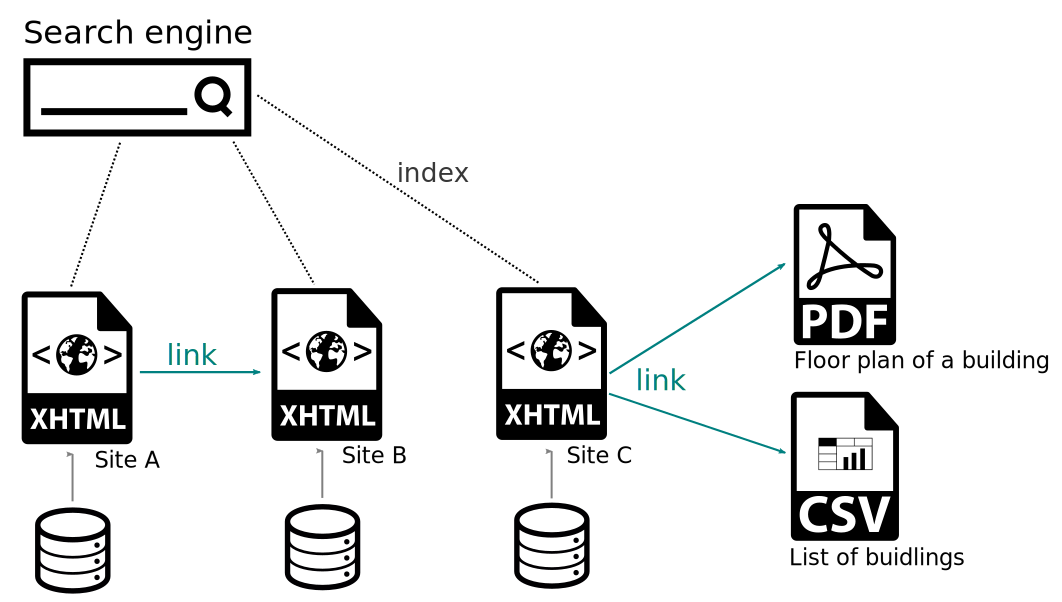
\includegraphics[width=0.75\textwidth]{graphics/webOfDocuments.png}
    \caption{Illustration of the Web of Documents}
    \label{fig:motiviation-web-of-documents}
\end{figure}

The same applies at the moment to the \gls{tuv}. In order to find a special location like a certain lecture hall and how it can be accessed without obstacles like stairways for persons with mobility-impairments, one has to search for information on different web sites, scan floor plans and eventually construct a convenient route to the location based on the gathered knowledge. For humans this procedure does not constitute a problem, but think of machines. The process of information retrieval through data mining or harvesting is quite difficult and/or time consuming. As a consequence application developers that may have innovative ideas, which would be a benefit for the information environment of the university, face a barrier that is hard to overcome. \gls{ld} is one way to transform this information published on multiple web sites into a university-wide data space (see figure \ref{fig:motiviation-web-of-data}).

\begin{figure}[h]
    \centering    
    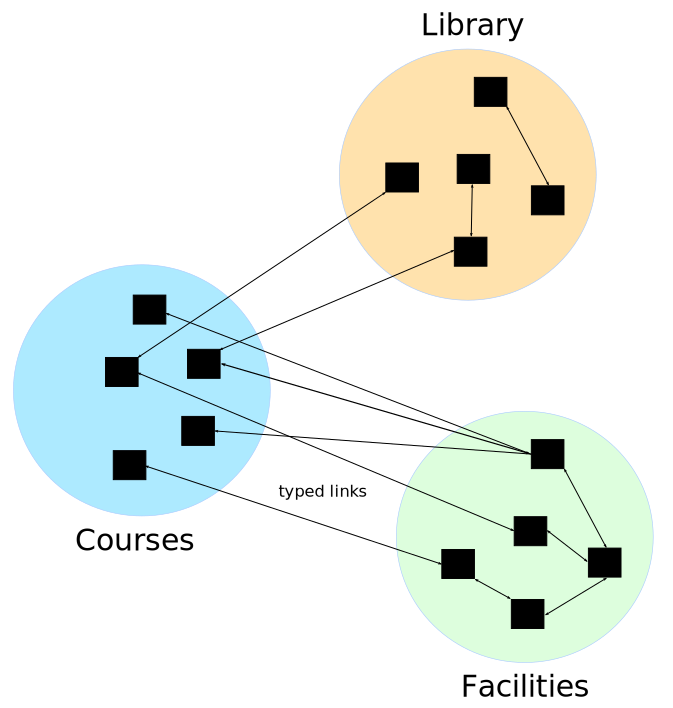
\includegraphics[width=0.5\textwidth]{graphics/webOfData.png}
    \caption{Illustration of the Web of Data}
    \label{fig:motiviation-web-of-data}
\end{figure}

\begin{quote} \gls{ld} describes a method of publishing structured data so that it can be interlinked and become more useful. It builds upon standard Web technologies, but rather than using them to serve web pages for human readers, it extends them to share information in a way that can be read automatically by computers. This enables data from different sources to be connected and queried
\cite{bizer_linked_2009}.\end{quote}

This thesis aims to show the potential that could evolve, if spatial data about \gls{tuv} is transformed into a machine-readable form such as \gls{ld}, by proposing a prototype of a map application based on a subset of spatial data about \gls{tuv}. This subset is intended to comply with the principles of \gls{ld} \cite{berners-lee_linked_2009} and to fulfil the submission criteria to the Linking Open Data cloud\footnote{\url{http://lod-cloud.net/}}, which are as follows \cite{cyganiak_linking_2011}:

\begin{itemize}
	\item There must be resolvable \texttt{http://} (or \texttt{https://}) URIs.
	\item They must resolve, with or without content negotiation, to RDF data in one of the popular RDF formats (RDFa, RDF/XML, Turtle, N-Triples).
	\item The dataset must contain at least 1000 triples.
	\item The dataset must be connected via RDF links to a dataset that is already in the diagram. This means, either your dataset must use URIs from the other dataset, or vice versam. We arbitrarily require at least 50 links.
	\item Access of the entire dataset must be possible via RDF crawling, via an RDF dump, or via a SPARQL endpoint.
\end{itemize}


\section{Problem description}
\label{intro-problem-description}

As already mentioned does the \gls{tuv} distribute spatial information over different sources. Few of this spatial data is actually in a machine-readable format, so that it can be transformed into \gls{ld} automatically. The \textbf{\textit{1st problem}} to solve is therefore the transformation process of the unstructured part of the data into a machine-readable format. Section \ref{solution-data-acquisition} is suggesting a solution for this problem.

The \textbf{\textit{2nd problem}} is how the structured spatial data shall be described so that it can be easily used by application developers as well as integrated into the Web of Data. The developed ontology shall be compliant to the best practises for publishing ontologies \cite{berrueta_best_2008}. Section \ref{solution-ontology-prototype} is suggesting a prototype of an ontology by taking already existing approaches (see section \ref{related-work-geospatial-ontologies} and \ref{related-work-indoor-modelling}) into consideration.

After the spatial data was transformed into \gls{ld}, a system must be designed to expose this data on the Web in order to qualify as \gls{lod}, representing the \textbf{\textit{3rd problem}} to solve. The solution shall take best practises for publishing \gls{ld}\cite{hyland_best_2014} and best practises for spatial data on the Web\cite{tandy_spatial_2016} into consideration. Section \ref{solution-architectural-prototype} is proposing an architectural prototype of such a system.

The \textbf{\textit{4th problem}} is the development of a map application that is based on the resulting \gls{lod}. The application shall answer the following question: \textit{"Give me all learning rooms that are nearby that are free in a given time range and are accessible without obstacles for person with mobility-impairments"} to show the potential of the data. Section \ref{solution-map-application} presents a solution to this problem.

\section{Structure of the thesis}
This chapter outlined the motivation for writing this thesis and gave a description of the problems for which a solution will be suggested. The rest of this thesis is structured as follows: Chapter \ref{background-chapter} discusses the basic concepts, principles and technologies that build the foundation of \gls{ld} and the Semantic Web. It is intended to be a brief introduction for readers that are not familiar with this topic. Chapter \ref{related-work-chapter} provides a summary of past efforts in research and works related to the focus of this thesis. In the subsequent chapter \ref{solution-chapter} a solution for the given problems will be suggested and discussed. This includes the prototype of an ontology that models the problem domain as well as an architectural prototype of a system that manages a subset of spatial data about the \gls{tuv} in form of \gls{ld} and provides a human- and machine-friendly interface to it. Finally, the implemented solution is evaluated and conclusions are drawn in the last chapter \ref{discussion-chapter}. It provides furthermore an outlook to future work and potential improvements. 

\chapter{Background}
\label{background-chapter}

\section{Web of Data}
\todo{Enter your text here.}

\section{RDF}
\gls{rdf}
\todo{Enter your text here.}

\section{Ontology}
\todo{Enter your text here.}

\subsection{RDFS}
\todo{Enter your text here.}

\subsection{OWL}
\todo{Enter your text here.}

\section{SPARQL}
\gls{sparql}
\todo{Enter your text here.}

\chapter{Related Work}
\label{related-work-chapter}

In this chapter important efforts and research related to this thesis are outlined. Section \ref{related-work-geospatial-ontologies} describes and evaluates geospatial ontologies that were suggested by \cite{tandy_spatial_2016} or discovered in the dataset of \gls{lov} through a systematic search. Section \ref{related-work-map-app} lists already existing map applications that are based on \gls{lod} and describes their capabilities. The final section \ref{related-work-indoor-modelling} describes done research and designed ontologies for modelling indoor environments.

\section{Geospatial ontologies}
\label{related-work-geospatial-ontologies}
This section is going to outline common ontologies for describing geospatial data and to evaluate them from the perspective of the given problem description (see \ref{intro-problem-description}).The ontologies were either be suggested by \cite{tandy_spatial_2016} or discovered in the dataset of \gls{lov} by common spatial search terms like \textit{'feature'}, \textit{'geometry'} or \textit{'location'}. \textit{Feature} and \textit{Geometry} are widely used terms in these ontologies and describe two different concepts of geospatial science. A \textit{feature}  is simply a spatial entity that can be everything from a building with fixed position to a movable food truck as long as it has a spatial extent. \textit{Geometry} as the name suggests is a certain geometric shape from points, lines to polygons. Geometric shapes can be used to describe  the spatial extent of \textit{features}.

The ontologies are visualized using the VOWL2 notation\cite{lohmann_vowl_2014}. Classes are modelled as circles, properties in form of rectangles; data type properties have a green colour and object properties a blue one. Literals are presented in a yellow rectangle.

\subsection{Basic Geo Vocabulary (WGS84)}
\label{related-work-geospatial-ontologies-wgs84}

\gls{geo}\cite{brickley_basic_2003} is a lightweight ontology published by W3C to describe the position of a spatial \textit{feature} using the WGS84 geodetic reference datum\footnote{\url{http://en.wikipedia.org/wiki/World_Geodetic_System}} with the properties \texttt{longitude}, \texttt{latitude} and \texttt{attitude}. The general class \texttt{SpatialThing} is the domain of all these properties. Figure \ref{fig:related-work-geospatial-ontologies:wgs84} shows a visualization of this ontology.

\begin{figure}[H]
    \centering    
    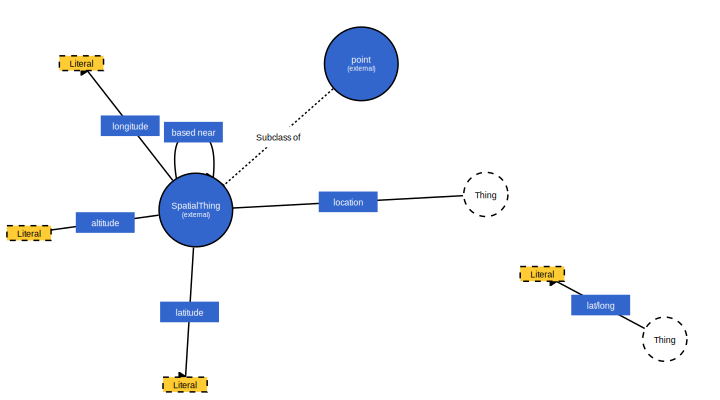
\includegraphics[width=\columnwidth]{graphics/vocabularies/wgs84.png}
    \caption{Visualization of \gls{geo}}
    \label{fig:related-work-geospatial-ontologies:wgs84}
\end{figure}

Advantages are its simplicity and popularity as an analysis of the \textit{Comprehensive Knowledge Archive} (CKAN, "The Data Hub"\footnote{\url{http://thedatahub.org}}) indicates. This analysis shows that \gls{geo} is used in \textbf{538} different datasets in the archive and is thereby the 4th most used ontology regarding usage in different datasets \cite{research_group:_akws_lodstats_????}. It is used by big players like DBpedia\footnote{\url{http://dbpedia.org}}, LinkedGeoData\footnote{\url{http://linkedgeodata.org/About}} and GeoNames\footnote{\url{http://linkedgeodata.org/About}}. 
Listing \ref{lst:related-work-geospatial-ontologies:wgs84-dbpedia} shows a data snippet of DBpedia describing the town square 'Karlsplatz' in Vienna with \gls{geo}.

\begin{lstlisting}[frame=single, caption=Snippet of DBpedia, label={lst:related-work-geospatial-ontologies:wgs84-dbpedia}]
@prefix dbr:  <http://dbpedia.org/resource/> .
@prefix geo:  <http://www.w3.org/2003/01/geo/wgs84_pos#> .

dbr:Karlsplatz  rdf:type  geo:SpatialThing ;
  rdfs:label  "Karlsplatz"@en , "Karlsplatz (Wien)"@de ;
  geo:lat     "48.19916534423828125"^^xsd:float ;
  geo:long    "16.370000839233398438"^^xsd:float .
\end{lstlisting}

\gls{geo} evolved into a standard for presenting the location of points of interest and as described by \cite{hyland_best_2014} in an article about best practises, standardized ontologies shall be used wherever possible to facilitate
inclusion into the Web of Data.

However, this ontology is not sufficient for describing spatial data more complex than a single point in a coordinate reference system.

\subsection{NeoGeo Geometry/Spatial Ontology}
\gls{ngeo}\footnote{\url{http://geovocab.org/geometry}} is an ontology that aims to provide a comprehensive descriptive power for modelling geographic regions, whereas \gls{spatial}\footnote{\url{http://geovocab.org/spatial}} aims to describe topological relationships between \textit{features}. Both ontologies were designed to have a strict distinction between \textit{features} and \textit{geometries} \cite{norton_neogeo_2012}.

\subsubsection{\gls{ngeo}} 
\gls{ngeo} follows the principle of modelling geometries in pure \gls{rdf}, which leads to a number of classes and properties for covering all shapes suggested by Simple Features Profile\footnote{\url{http://www.ogcnetwork.net/gml-sf}}. This includes points, lines and polygons. Shapes that go beyond a simple point are represented by a \gls{rdf} collection of \texttt{point} instances, whereby \texttt{point} is a external class of \gls{geo}. Figure \ref{fig:related-work-geospatial-ontologies:ngeo} shows a visualization of this ontology.

\begin{figure}[h]
    \centering
    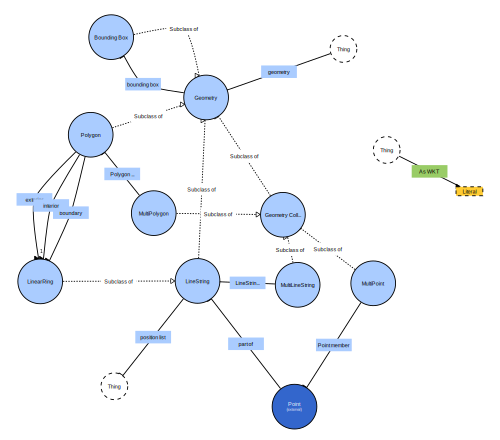
\includegraphics[width=1.0\textwidth]{graphics/vocabularies/geom.png}
    \caption{Visualization of \gls{ngeo}}
    \label{fig:related-work-geospatial-ontologies:ngeo}
\end{figure}

One advantage of this approach is that triple stores do not have to meet special requirements in order to enable the querying over geometric data like it is the case for GeoSPARQL. However, this shifts the burden of writing geometric queries to developers. A further problem is the high demand for resource identifiers or blank nodes (at least for each point of a shape), as the example of describing the geometry of Iceland shows\footnote{\url{http://nuts.geovocab.org/id/IS_geometry.ttl}}; this significantly increases the verbosity of the data without adding particular gains of expressitivity to it\cite{battle_geosparql:_2011}. \gls{ngeo} has also a generic property \texttt{asWKT} for pointing to the \gls{wkt} serialization of a geometry, which has at the moment of writing the status 'deprecated'.

LinkedGeoData uses the \texttt{geometry} property of this ontology to point to the \textit{geometry} of a \textit{feature}, but the \texttt{asWKT} property of GeoSPARQL to represent the geometry.

\subsubsection{\gls{spatial}}
\gls{spatial} is an ontology that aims to provide properties to make topological relationships of \texttt{features} explicit, which else would only exist implicit in the geometric data. Included properties cover all topological relationships described by RCC-8 like does a \textit{feature} overlap with another \textit{feature}. One problem of making the relationships explicit is that these relationships have to be adopted if the \textit{geometry} of \textit{features} changes.

\subsection{GeoSPARQL}
GeoSPARQL defines a set of \gls{sparql} extension functions, a set of \gls{rif} rules, and a core ontology for geographic information\cite{perry_ogc_2012}. ``GeoSPARQL attempts to unify data access for the geospatial Semantic Web""\cite{battle_geosparql:_2011}. Figure \ref{fig:related-work-geospatial-ontologies:geosparql} shows a visualization of this core ontology. It has two major classes namely \texttt{Feature} to represent spatial \textit{features} and \texttt{Geometry} to represent \textit{geometries}. An instance of \texttt{Geometry} can be assigned to an instance of \texttt{Feature} with the property \texttt{hasGeometry}. It is based on the Simple Features model\footnote{\url{http://www.ogcnetwork.net/gml-sf}} like \gls{ngeo}. However, GeoSPARQL defines two properties that can be used to point to the serialization of a geometry; either \texttt{asWKT} for \gls{wkt} or \texttt{asGML} for \gls{gml}; in contrast to \gls{ngeo}, where \textit{geometries} are represented in pure \gls{rdf}. The fact that \textit{geometries} are serialized using \gls{wkt} or \gls{gml} simplifies the integration of \textit{geometries}, because these serialization formats are widely supported (e.g. QGIS). GeoSPARQL proposes furthermore a set of extension functions that can be separated into two categories. The first category includes functions that take a number of \textit{geometries} as arguments and produces a new one or returns a value with a certain datatype. The distance function for instance takes two \textit{geometries} as well as a reference to measurement unit like meters and returns a \texttt{xsd:double} value. The second category are functions that are equivalent to the properties describing topological relationships (e.g. contains, coveredBy), only that these functions can be used in filters and are computed on-the-fly; not asserted in the knowledge base. However, the used triple store or \gls{ld} framework must support those functions and the GeoSPARQL standard in general, which limits the choice. As it will be discussed in section \ref{solution-architectural-prototype:rdf-framework}, one of the common frameworks Apache Jena and its native triple store is at the moment not compliant with the GeoSPARQL standard. 

\begin{figure}[h]
    \centering
    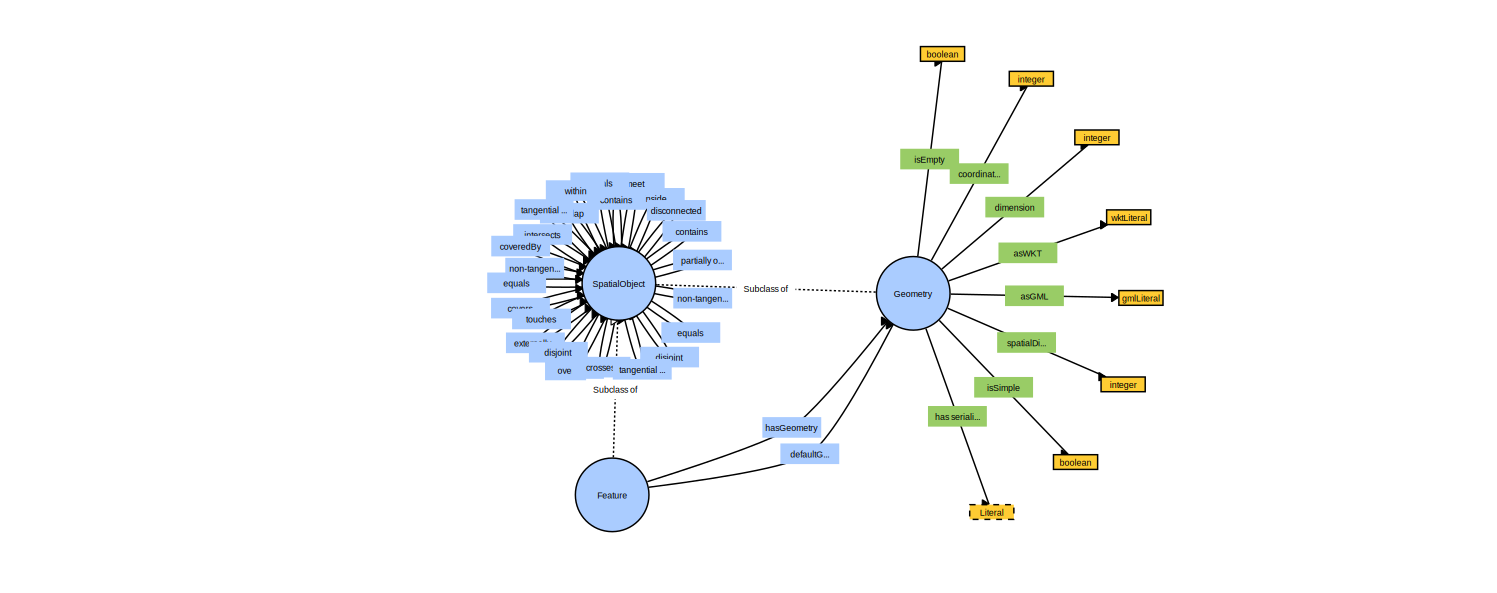
\includegraphics[width=1.0\textwidth]{graphics/vocabularies/geosparql.png}
    \caption{Visualization of GeoSPARQL}
    \label{fig:related-work-geospatial-ontologies:geosparql}
\end{figure}

\subsection{schema.org}
schema.org\footnote{\url{http://schema.org/}} is an initiative that was started by Google, Bing and Yahoo! (subsequently joined by Yandex) to promote a common ontology for publishing structured data mark-up on web pages \cite{guha_introducing_2011}. This machine-readable information can then be extracted from web pages by search engines to improve search results.

schema.org is a quite broad ontology covering a set of different domains from events, organizations to places. For this thesis especially the class \texttt{Place} is of interest describing entities with a fixed, physical extent; it has a set of more specific subclasses. This class has properties to assign an address to its instances  (\texttt{address}) as well as to provide geo-information (\texttt{geo}). The value of the property \texttt{geo} can either be instances of the class \texttt{GeoCoordinates} or \texttt{GeoShapes}. \texttt{GeoCoordinates} represents a point in a georeference system similar to \gls{geo}. \texttt{GeoShapes} on the other hand provide the ability to describe more complex geometric shapes including cirlces, boxes, polygons and simple lines. All those shapes are expressed in textual form following an own specific pattern, in contrast to GeoSparql, which declares the use of \gls{gml} or \gls{wkt}. However, such literals could be transformed into \gls{wkt} by string operations (supported in \gls{sparql}) except for the circle, which has no direct representation in \gls{wkt}.

One advantage of this ontology is the visibility to search engines when exposed on web pages in one of the supported formats (Microdata\footnote{\url{https://www.w3.org/TR/microdata/}}, \gls{rdfa}\footnote{\url{https://www.w3.org/TR/rdfa-syntax/}} and JSON-LD\footnote{\url{http://json-ld.org/}}). As mentioned earlier, the embedded data can then be extracted and in fact major search engines crawl for it to enhance search results\cite{haas_enhanced_2011}. However, there are odd ascriptions of properties like that instances of the class \texttt{Beach} (subclass of \texttt{Place}) can have the property \texttt{faxNumber}; it must be considered that schema.org is meant for web masters to add structured metadata to their web sites \cite{veres_schema.org_2013} and not to describe a specific domain precisely.

\subsection{ISA Programme Location Core Vocabulary}
\gls{locn} is an ontology that provides a set of properties and classes to describe the geometry, address and location of a \textit{feature}. Figure \ref{fig:related-work-geospatial-ontologies:locn} shows a visualization of this ontology. It provides a comprehensive set of properties to describe the address of a \textit{feature}, but a mininal set for geometries and locations. For geometries this ontology suggests the use of external classes or a simple literal representing the serialization of the geometry in formats such as \gls{wkt} and \gls{gml}. Those suggested classes are \textit{Geometry} of GeoSPARQL with its more specific subclasses and \texttt{GeoCoordinates} as well as \texttt{GeoShapes} from schema.org. In case of representing simple points also \texttt{point} of \gls{geo} is mentioned. \cite{perego_isa_2015} Howerver, this quite broad range of possibilities does not make it easy for the consumer of such \gls{ld}.

\begin{figure}[h]
    \centering
    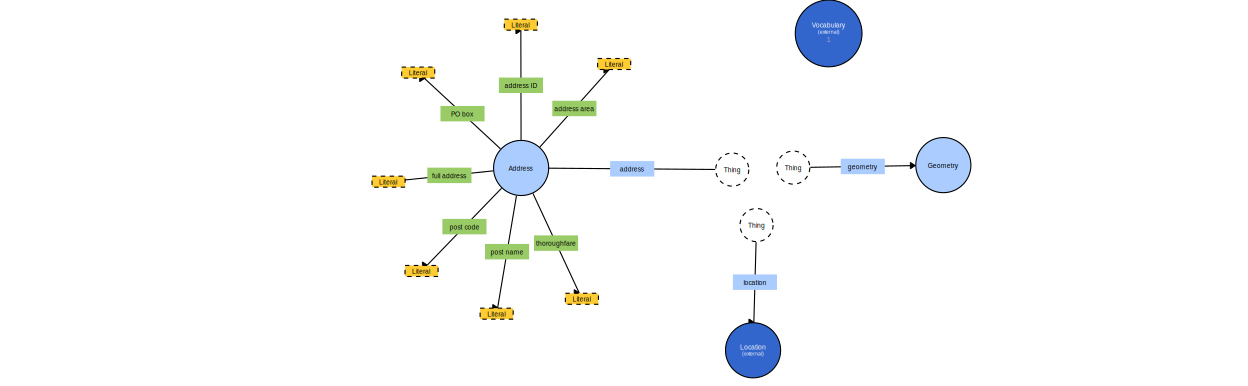
\includegraphics[width=1.0\textwidth]{graphics/vocabularies/locn.png}
    \caption{Visualization of \gls{locn}}
    \label{fig:related-work-geospatial-ontologies:locn}
\end{figure}


\section{Linked Open Data based map applications}
\label{related-work-map-app}

Multiple universities (e.g. Linked Universities\footnote{\url{http://linkeduniversities.org}}) exposed their public university data and map applications played out to be a common use case for this data.

University of Münster started an Open Data initiative named LODUM\cite{kesler_linked_2012} from which a map application\footnote{\url{http://app.uni-muenster.de/Karte/}} evolved that shows the location of buildings and which departments are located in the selected building, but there is no deeper insight into the buildings. However, there is a publication of the initiative that deals with the issue of indoor navigation \cite{kostic_automated_2015-1}. Furthermore an indoor map ontology named LIMAP\footnote{\url{http://lodum.de/results/}} was designed.

University of Southampton is a further university that exposed spatial information about their campus as \gls{lod}. In contrast to the map of the LODUM initiative Southampton`s map application\footnote{\url{http://maps.southampton.ac.uk/}} (see figure \ref{fig:related-work-map-app:southampton}) gives insight into buildings and shows the location of certain rooms with the ability to switch the floor. It shows also computer rooms with their current estimated capacity and opening hours.  

\begin{figure}[h]
    \centering
    \includegraphics[width=0.75\textwidth]{graphics/maps/southampton-map-app.png}
    \caption{Map application of University of Southampton}
    \label{fig:related-work-map-app:southampton}
\end{figure}

University of Oxford has also exposed spatial information in form of \gls{lod} on their Open Data portal and developed an application named \textit{University Science Area Map} \footnote{\url{https://data.ox.ac.uk/explore/science-area/}}. It highlights buildings, where departments of a certain field are located, on a map, but it gives no insight into the buildings.

\section{Indoor modelling}
\label{related-work-indoor-modelling}
Section \ref{related-work-geospatial-ontologies} outlined ontologies to describe the spatial extent of \textit{features} and topological relationships between them, but those ontologies are not intended for expressing the characteristics of \textit{features} in an indoor environment; like for example that a \textit{feature} is a learning room with certain opening hours or an elevator to get from one floor to another. This section discusses previous efforts and ontologies to model indoor environments and also how to navigate in them.

IndoorGML\footnote{\url{http://indoorgml.net/}} is a \gls{xml} schema of OGC that aims to provide a framework for representing and exchanging indoor spatial information, but no efforts has yet been made to transform its model to the \gls{ld} domain. OntoNav presents a semantic indoor navigation system that aims to follow a user-centric paradigm in which the capabilities, limitations and preferences of the user are taken into consideration for computing the best suiting path. A path is according to OntoNav a sequence of connected corridors, passages (stairways, ramps, elevators, etc.) and exits from one location to another\cite{anagnostopoulos_ontonav:_2005}. ONALIN is a ontology that models the indoor environment similar to OntoNav, but it follows the approach of modeling buildings as network of hallways consisting of different points (start, decision and corner points); resulting in a finer granularity. ONALIN also takes the American Disability Act into consideration, which leads to properties for describing the height and number of steps of stairways or the height of sinks in a restroom \cite{dudas_onalin:_2009}. Both ontologies are at the moment not locatable over the Web. iLoc is an ontology that has a minimal set of classes to describe the internal structure of a building from rooms, floors to vertical passages like elevators and stairways. Points of interest like entrances and landmarks play a special role in the navigation. A route section connects then two points and asserts that there is a walk-able path between them. This route section can have certain constraints like an access control measurement is required or steps have to be climbed \cite{szasz_ilocbuilding_2010}.


\subsection{Other ontologies}
\label{related-work-indoor-modelling-other-ontologies}
The ontologies mentioned in this section have been discovered in the repository of \gls{lov} by searching for terms such as \textit{'room'}, \textit{'building'} and \textit{'toilets'} or explored in datasets of map applications based on \gls{lod} (see section \ref{related-work-map-app}).

\gls{rooms} provides a minimal set of classes and properties to describe the basic structure of a building. It has 6 classes \texttt{Building}, \texttt{Floor}, \texttt{FloorSection}, which is a named (identifiable) section of a floor,\texttt{Room} and \texttt{Desk} as well as \texttt{Site}, which describes an area of land like a campus.

\chapter{Solution}
\label{solution-chapter}

This chapter suggests solutions for the given problem description (see \ref{intro-problem-description}). Section \ref{solution-data-acquisition} is dealing with the problem of transforming unstructured spatial data of the \gls{tuv} into a machine-readable format. The question of how this structured data shall be described is answered in section \ref{solution-ontology-prototype}, where a prototype of an ontology is discussed. The subsequent section \ref{solution-architectural-prototype} is proposing an architectural prototype of a system for integrating and publishing \gls{ld} consistent with the \gls{ld} principles \cite{berners-lee_linked_2009}. The final section \ref{solution-map-application} is presenting a map application to show the potential of the generated spatial \gls{lod}.

\section{Data acquisition}
\label{solution-data-acquisition}
Spatial data of the \gls{tuv} is distributed over multiple sources with different formats and data owners. In order to be eventually transformed into \gls{ld}, this data must be extracted and prepared for the transformation. Figure \ref{fig:solution-data-acquisition:sources} visualizes the different data sources.

The major source for building information is the web site of the facility management unit of the \gls{tuv} (GUT\footnote{\url{http://www.gut.tuwien.ac.at/}}). This site lists all buildings and an enumeration of their floors in form of a (X)HTML table. It also contains links to the floor plans that are provided as \gls{pdf} files as well as to a \gls{pdf} file for each building consisting of a table of all contained rooms with their intended function (e.g. office room, sanitary room). The central information system TISS\footnote{\url{https://tiss.tuwien.ac.at/}} provides a RESTful API that gives access to organizational information and the public address book. For this thesis, this API is useful for linking persons and organizations to their offices. TISS has also a web page dedicated to present the event schedule of certain rooms like lecture halls, but this data is not available over the mentioned RESTful API; only in a human-readable form.

Section \ref{solution-data-acquisition-tables} deals with the problem of extracting and transforming tables from \gls{pdf}s and web pages. The approach for processing floor plans is discussed in section \ref{solution-data-acquisition-floor-plans}. Tools for transforming \gls{xml} documents into \gls{ld} are outlined in section \ref{solution-data-acquisition-xml}.

\begin{figure}[h]
    \centering
    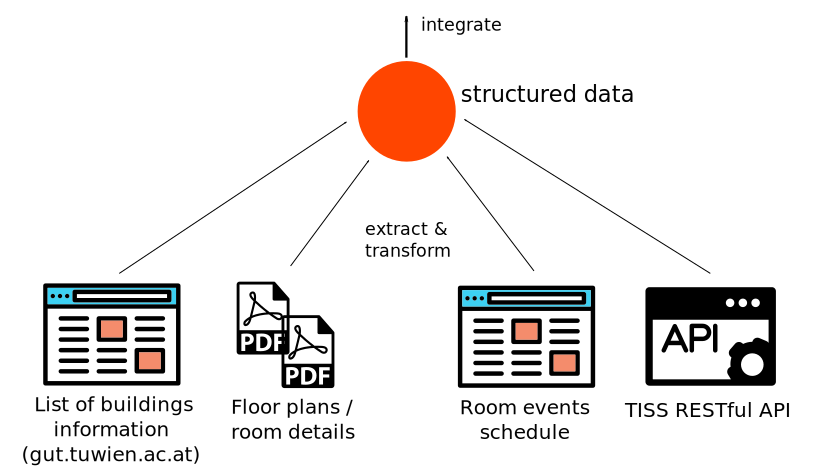
\includegraphics[width=0.75\textwidth]{graphics/dataAcquisitionSources.png}
    \caption{Visualization of the data sources}
    \label{fig:solution-data-acquisition:sources}
\end{figure}

\subsection{(X)HTML and \gls{pdf} tables}
\label{solution-data-acquisition-tables}
As mentioned earlier, some of the data is presented to users only in form of (X)HTML tables and must therefore be extracted in order to be transformed into \gls{ld}. Web scrapers/Web harvester are an useful tool to extract such tables from web pages manually or by using XPATH expressions and to store them in an intermediate representation. For this thesis a chrome extension named 'Web Scraper' \footnote{\url{http://webscraper.io/}} was used. This intermediate representation was then exported into a \gls{csv} file. 

For tables in \gls{pdf} files a different approach is required and the tool named 'Tabula'\footnote{\url{http://tabula.technology/}} is qualified for this kind of problem. It can detect tables automatically and transforms them into an intermediate representation, but this does not always work appropriately. In this case, the user can support the program by selecting the relevant parts manually. This intermediate representation was then also exported into a \gls{csv} file.

After the information was extracted from web pages and \gls{pdf} files and transformed into a structured format, it still was messy data that is not convenient for a further transformation into \gls{ld}. In this case the tool OpenRefine\footnote{\url{http://openrefine.org/}} is quite useful. It provides a set of functions to manipulate messy, tabular data including an own expression language named GREL. LODRefine and RDF extension are extensions for OpenRefine, which enable the transformation of tabular data into \gls{rdf} by mapping columns to classes and relationships between columns to properties. This mapping is then computed for each row. 

\subsection{Floor plans}
\label{solution-data-acquisition-floor-plans}
Floor plans are ideal for describing the internal structure of a building, but they are mostly available in form of images and vector graphics. This representation is fine for humans, but not for machines; because the floor plan should not only be available as single image, but rather be the knowledge base for applications to find paths and locate rooms in the corresponding building.

Google Maps is a map application that also gives insight into certain buildings. It provides a tool \footnote{\url{https://maps.google.com/floorplans/find}}, where any user can submit floor plans and this floor plan then will be automatically transformed into an internal representation that can thenceforward be looked at in the application (if accepted). The problem is that the user cannot demand access to this internal representation of the plan, although the user may be the owner. Figure \ref{fig:solution-data-acquisition:tuvienna-lib-gm-indoor} shows the indoor plan of \gls{tuv}`s main library in Google Maps.

\begin{figure}[h]
    \centering
    \includegraphics[width=0.75\textwidth]{graphics/google-maps-tu-vienna-library-indoor-plan.png}
    \caption{Google Maps: Indoor plan of \gls{tuv}`s main library}
    \label{fig:solution-data-acquisition:tuvienna-lib-gm-indoor}
\end{figure}

Due to the lack of alternatives, the approach used for this thesis was to manually transform one floor plan of one building into shape files. The tool used for this approach was the Open Source software QGIS\footnote{\url{http://www.qgis.org/}}. It has two plugins that are useful for the transformation, the 'Open Layers' plug-in to enable the use of OpenStreetMaps among others and the GDAL georeferencing plug-in to position a raster image on a map. Especially the last plug-in is important for positioning the floor plan to the correct position on the map, whereby the map should already contain the boundary of the building. After georeferencing the floor plan, a shape file of the rooms and other \textit{features} of interest can be created. Each of the created shapes has a table of attributes with an unique ID that can be set by the user. The unique ID of each shape is an \gls{iri}, so that the shape is ready to be transformed into \gls{ld}. The resulting shape file can then be exported in multiple formats including GeoJSON\footnote{\url{http://geojson.org/}}. For this thesis, a \gls{csv} file with the \gls{wkt} serialization of each shape of the file and the corresponding ID per row showed to be the easiest way to integrate this data. Figure \ref{fig:solution-data-acquisition:tuvienna-lib-gm-indoor} shows a shape file of rooms on the basement floor of the informatics institute`s building at the \gls{tuv}.

\begin{figure}[h]
    \centering
    \includegraphics[width=0.75\textwidth]{graphics/qgis-floor-plan-building-h-eg.png}
    \caption{Room shapes file of the basement floor of the informatics institute`s building}
    \label{fig:solution-data-acquisition:tuvienna-lib-gm-indoor}
\end{figure}

\subsection{\gls{xml}}
\label{solution-data-acquisition-xml}

The RESTful API of the central information system TISS returns results of its services  either in form of an \gls{xml} document or \gls{json}. Thus the responses are already in a (semi-)structured format; the question is how to transform this data into \gls{ld}. \gls{xslt} offers an useful language for transforming a source \gls{xml} document into a target document that could be likewise an \gls{xml} document or other representations like plain text or HTML.  The data-management layer (see section \ref{solution-architectural-prototype:ld-management}) of the proposed system uses this language therefor to transform a \gls{xml} document with a known schema into a RDF/XML document, which expresses \gls{rdf} data as an \gls{xml} document. GRDDL\cite{connolly_gleaning_2007} can be used to mark parts of \gls{xml} documents with pointers to \gls{xslt} stylesheets, but this has to be implemented by the API designers.

\section{Prototype of ontology}
\label{solution-ontology-prototype}
In this section two ontologies will be proposed that are intended to cover the specific domain of spatial university data. Section \ref{solution-ontology-prototype:spatial} presents an ontology for describing the campus from buildings to indoor environments, whereas section \ref{solution-ontology-prototype:navigation} proposes an ontology for modelling indoor navigation. The design process took best practises for publishing ontologies\cite{berrueta_best_2008} into consideration. In order to enhance the interchangeability of the described data it is commonly understood to reuse terms of common ontologies, which is why chapter \ref{related-work-chapter} outlined common geospatial ontologies as well as ontologies and approaches for modelling indoor environments. The conclusion of the evaluation was to use the GeoSPARQL ontology for describing the geometry of indoor features and buildings. Hence, the system architecture has to consider an additional prerequisite; the used triple store should support the GeoSPARQL extensions and for the purpose of better scalability also spatial indexing.

\subsection{Spatial ontology}
\label{solution-ontology-prototype:spatial}

\todo{describe ... }

\subsection{Navigation ontology}
\label{solution-ontology-prototype:navigation}
The spatial ontology (see section \ref{solution-ontology-prototype:spatial}) provides the necessary expressiveness to describe the indoor environment of buildings from rooms, corridors to entrances, but no assertions can be made about how this \textit{features} are actually connected. Some conclusion can be drawn by looking at the \textit{geometries} of \textit{features}. In order to get for example the two rooms a door is connecting, the distance to the \textit{geometry} of all rooms must be computed and the two rooms with the lowest distance by considering a reasonable threshold (in case one or both rooms are unknown) could be selected. Furthermore, would it be possible to compute the path to a room by considering the \textit{geometries}, but this would still need information about how certain \textit{features} are connected. A door for example could require an access control measure to pass it in one direction, but in the other direction it could be passed without constraints. A further problem to consider, if the path should be computed based on the \textit{geometries}, is that not all paths may be accessible for all persons. A space could contain steps that are hard to overcome for persons with mobility impairments, or the space could be occupied by other obstacles.  As an example, directly in front of or behind a door could be some steps that would force such persons to use another entrance.

For this thesis the approach of pre-defining routes based on \textit{features} and points of interest was chosen for the purpose of simplification. However, the previous mentioned techniques could be used to compute certain parts of the route and humans can take over, when it became more complex. Another important question to address is the granularity. Should a route consists of a collection of connected rooms, horizontal passageways like corridors and vertical passageways like elevators or be more detailed with different paths inside of rooms and corridors. The problem of the first approach is that there could be some obstacles inside of rooms and corridors (e.g. steps in the middle of the corridor) that would be overseen. In case of the more detailed routes consisting of a collection of points of interest such obstacles can be taken into consideration, but consequently leads to more verbose data than with the first approach.

Figure \ref{fig:solution-ontology-prototype:navigation} shows the designed ontology for the indoor navigation. It has two major classes named \texttt{NavigationEntity} and \texttt{Constraint}. The class \texttt{NavigationEntity} has two subclasses namely \texttt{Route} and \texttt{Access}.

\begin{figure}[h]
    \centering
    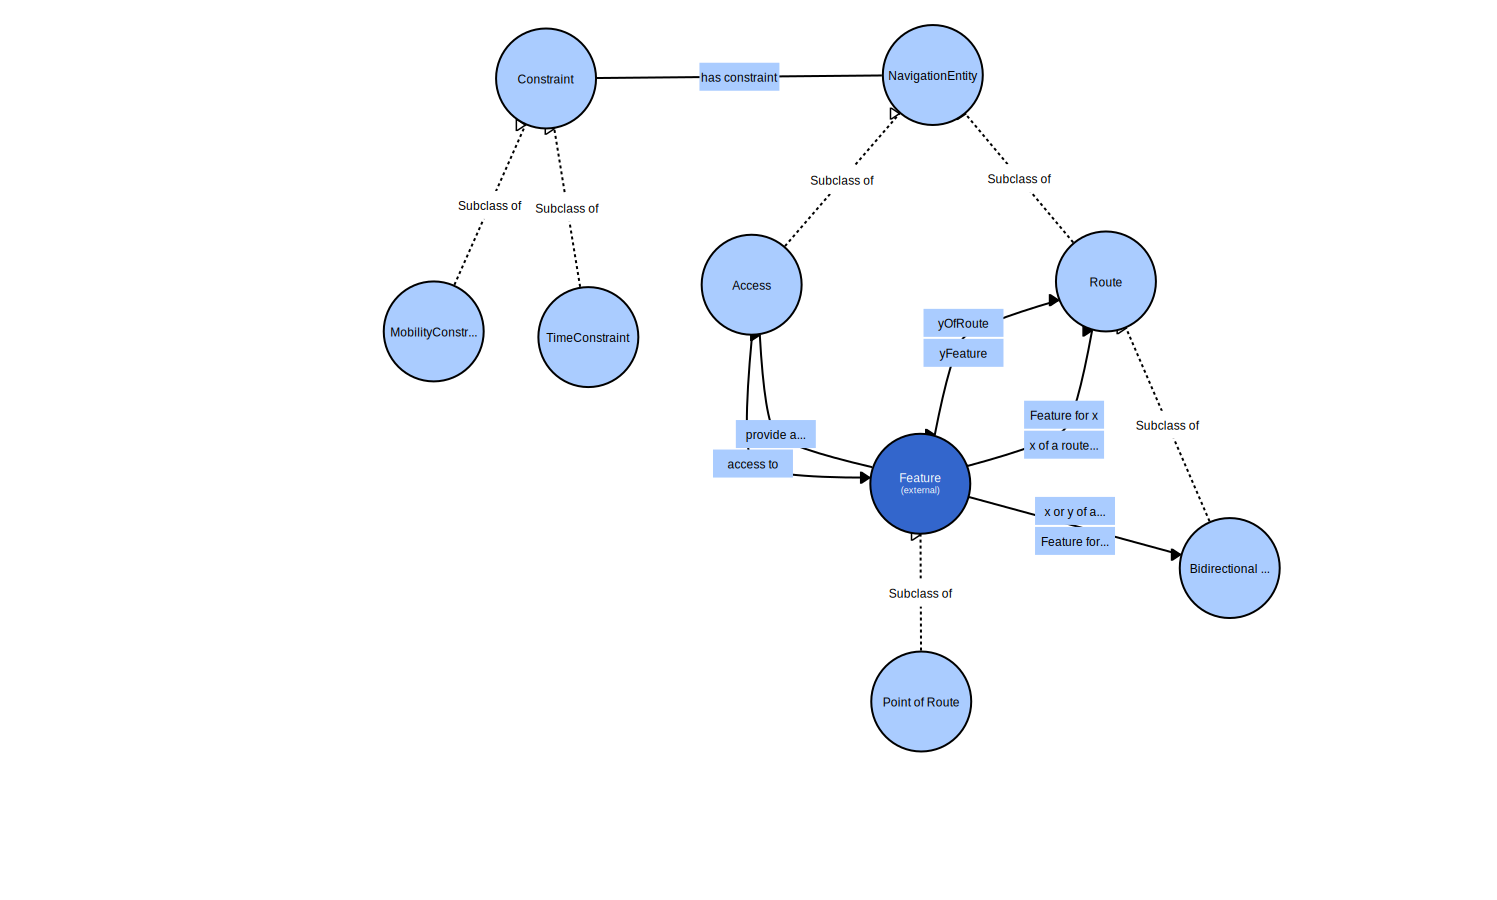
\includegraphics[width=0.8\textwidth]{graphics/solution/ontology/tuViennaNavigationOntology.png}
    \caption{Visualization of the navigation ontology}
    \label{fig:solution-ontology-prototype:navigation}
\end{figure}

\paragraph{Route} is a path R(x,y) between two spatial \textit{features} x and y, whereby x and y are instances of the class \texttt{Feature} of GeoSPARQL. The path is walk-able from x to y by considering the given constraints of this route. No assumptions about the other direction R(y,x) are made. The x and y values of a route are assigned to it by the properties \texttt{xOfRoute} (inverse property \texttt{xFeature}) and \texttt{yOfRoute} (inverse property \texttt{yFeature}). A door that requires an access control measurement in one direction and not in the other is one example of a \texttt{Route}.

\subparagraph{BiRoute} is a subclass of \texttt{Route} and represents a path R(x,y) between two spatial \textit{features}, whereas the path between x and y is walk-able in both directions considering the given constraints. The values x and y can be assigned to an instance of \texttt{BiRoute} by using the property \texttt{xyOfRoute} (inverse property \texttt{xyFeature}). This property is a subproperty of \texttt{xOfRoute} and \texttt{yOfRoute}; means that each value of \texttt{xyOfRoute} is automatically x and y of a \texttt{Route}. Consequently also R(x,x) and R(y,y) are valid paths, which must be filtered. A simple path inside of a corridor is an example for a \texttt{BiRoute}.

It would be nice to query for the path between two spatial \textit{features} in pure \gls{sparql}. The most recent version of the language (v1.1) introduced a new feature called property paths. These property paths can be used to recursively follow property links\cite{harris_sparql_2013}. However, property paths lack expressivness and queries that count the number of possible paths between two nodes or compute the shortes path are not expressible with \gls{sparql} v1.1 \cite{reutter_recursion_2015}\cite{atzori_computing_2014}. Nonetheless, a \gls{sparql} query could prepare the input for a path finding algorithm. 

\begin{lstlisting}[language=sparql, frame=single, basicstyle=\footnotesize, caption=Prepare for path finding, label={lst:solution-ontology-prototype:navigation:prepare}]
SELECT ?xRouteFeature ?route ?yRouteFeature ?length WHERE
{
    values (?startFeature ?endFeature) {
    	(<http://finder.tuwien.ac.at/spatial/accessunit/id/HEEGM1> 
    	<http://finder.tuwien.ac.at/spatial/elevator/id/HFEG02C>)
    }
    # Fetch the features of possible paths
    ?startFeature (navi:xOfRoute/navi:yFeature)+ ?routeFeature .
    ?xRouteFeature navi:xOfRoute ?route ;
    	gsp:hasGeometry [ gsp:asWKT ?xRouteFeatureGeom ] .
    ?route navi:yFeature ?yRouteFeature .
    ?yRouteFeature (navi:xOfRoute/navi:yFeature)* ?endFeature ;
      	gsp:hasGeometry [ gsp:asWKT ?yRouteFeatureGeom ] .
    FILTER(?xRouteFeature != ?yRouteFeature).
    # Computes the length of the path in meters.
    BIND(gspf:distance(?xRouteFeatureGeom, ?yRouteFeatureGeom, uom:metre)
    	as ?length) .
    # Remove all routes that have certain constraints.
    FILTER NOT EXISTS {
    	?route navi:hasConstraint ex:building-id-H-opening-hours .
    }
}
\end{lstlisting}

Listing \ref{lst:solution-ontology-prototype:navigation:prepare} shows a query returning a result set of all \textit{features} (xRouteFeature) that are part of a possible path between two given \textit{features} (startFeature, endFeature) and all the adjacent, noteworthy \textit{features} (yRouteFeature) for each of them. An adjacent \textit{feature} (yRouteFeature) is noteworthy, if there is a possible path to the target \textit{feature} (endFeature) and the route R(xRouteFeature, yRouteFeature) has no undesirable constraints. Additionally, the length will be determined for each route in order to have a weight for the path finding algorithm. The length is simply the distance between the x- and y-\textit{feature} of a route.

\subparagraph{Access} ...

\todo{finish ... }

\section{Architectural prototype}
\label{solution-architectural-prototype}

This section proposes a architectural prototype of a software system that manages spatial \gls{lod} from integration to publication. Figure \ref{fig:solution-architectural-prototype} shows an overview of this architecture, which is separated into three layers; the data management, service and presentation layer. The shown data sources (described in section \ref{solution-data-acquisition}) build the knowledge base of the system. Section\ref{solution-architectural-prototype:ld-management} discusses the data management layer, which deals with the integration of those data sources and the maintenance of it. The linking of the local spatial \gls{ld} with external sources like LinkedGeoData and GeoNames is described in section \ref{solution-architectural-prototype:linking}. After the local spatial data has been integrated into the system, the resulting \gls{ld} can be published. Section \ref{solution-architectural-prototype:ld-publishing} discusses different approaches for the publication with the goal to make the underlying \gls{ld} easily accessible by machine and human agents. The prototype of a map application that make use of the provided services of the system is presented in the subsequent section \ref{solution-map-application}.   

In order to implement the suggested prototype the programming language Java was used and section \ref{solution-architectural-prototype:rdf-framework} outlines the common frameworks for handling \gls{ld} in this language. It also describes the reasoning, why RDF4J\footnote{\url{http://rdf4j.org/}} was chosen.

\begin{figure}[h]
    \centering
    \includegraphics[width=1.0\textwidth]{graphics/finderArchitecture.png}
    \caption{Overview of the system architecture}
    \label{fig:solution-architectural-prototype}
\end{figure}

\subsection{RDF Framework}
\label{solution-architectural-prototype:rdf-framework}
Handling \gls{rdf} data (as representation of \gls{ld}) is an essential part of the proposed software system and a reliable framework for fulfilling this task is needed. Besides reliability the framework should also support most of the following requirements:

\begin{enumerate}
	\item it should be freely available, favourably Open Source.
	\item it should be possible to store data into either an embedded or external triple store.
	\item it should support \gls{sparql} to query data.
	\item it should support common serialization formats like RDF/XML, Turtle, LD-JSON and N-Triples.
	\item it should support spatial functionalities in \gls{sparql} queries compliant to GeoSPARQL (see section \ref{related-work-geospatial-ontologies}). At least the minimal distance between two geometries must be computable.
	\item it should be possible to reason over stored \gls{ld} given a list of ontologies. 
\end{enumerate}

There are currently two common frameworks for handling \gls{rdf} data in the Java environment namely Apache Jena\footnote{\url{https://jena.apache.org/}} and Sesame, which has recently been migrated to the project RDF4J\footnote{\url{http://rdf4j.org/}}. Both are Open Source, but none fulfils all of the mentioned requirements, why it is also necessary to take plug-ins and external triple stores into consideration.

\paragraph{Apache Jena} is a framework that can be used to store, manipulate and query \gls{ld}. Its architecture consists basically of three layers, the store API at the bottom, the inference API in the middle, the RDF API and  SPARQL API respectively as interface to the application code \cite{the_apache_software_foundation_jena_????}. In contrary to RDF4J, \gls{rdf} data can be parsed into a model instance and thenceforward this model can be used to query and reason over it. RDF4J requires this \gls{rdf} data to be at least stored into a repository embedded in memory in order to be queried using \gls{sparql}. One advantage of Jena over RDF4J is also the built-in reasoner that supports simple \gls{rdfs} reasoning as well as multiple profiles of \gls{owl} \cite{the_apache_software_foundation_jena_????-1}. Jena supports different types of storage from native triple store to a memory based one; also custom triple stores can be used, but in this case an adopter is required. In case of spatial functionalities Jena does support spatial relationships like near by, within box, intersect box or north/south/west/east of \cite{the_apache_software_foundation_spatial_????}, but it is not compliant to the GeoSPARQL standard . Functions like computing the minimal distance between two geometries are not covered. There is also no support for \gls{gml} serializations of geometries. As a consequence requirement \textbf{\textit{5}} is not fulfilled. A way to circumvent this problem is to use an external triple store that provides these spatial functionalities, but as mentioned above this triple store must offer an adaptor for Jena, which limits the number of considerable triple stores.
 
\paragraph{RDF4J} is as well a framework to store, manipulate and query \gls{ld}, but there are conceptual differences. As mentioned above in RDF4J actions are carried out against repositories and a model has less functionality than in Jena; it is simply a collection of statements (triples). RDF4J provides \gls{rdfs} reasoning, but nothing more expressive than that. However, custom reasoners can be added like in Apache Jena too. An advantage of RDF4J over Jena is the simplicity of adding other storages besides the built-in ones (from native triple stores to in-memory repositories). It provides for example classes to use a \gls{sparql} endpoint as repository. In fact there are multiple external triple stores that can be used with RDF4J over HTTP like GraphDB\footnote{\url{http://ontotext.com/products/graphdb/}}, Stardog\footnote{\url{http://docs.stardog.com/}} or Blazegraph\footnote{\url{https://www.blazegraph.com/product/}}. RDF4J does have a package named \texttt{rdf4j-queryalgebra-geosparql} to add spatial functionalities compliant with GeoSPARQL, but during testing the minimal distance function always returned null. It was not clear, if there was a bug in the framework or it was used incorrectly. This leads to a major drawback of RDF4J in contrast to Jena, it has a sparse documentation at the moment of writing.

\subsubsection{Conclusion}

The support of spatial functionalities in \gls{sparql} queries like computing the minimal distance between two geometries is crucial for the proposed software system, not only for the navigation task, but also for spatial linking of resources to external sources (see section \ref{solution-architectural-prototype:linking}). In this regard both frameworks would be insufficient, but custom/external triple stores can help here. GraphDB is a triple store that is able to take care of reasoning (with support of \gls{rdfs} as well as profiles of \gls{owl}). Additionally, it offers a GeoSPARQL plug-in that not only adds the corresponding spatial functionalities, but also spatial indexing resulting in a performance gain. This is the reason why RDF4J was chosen as framework, because it is easier to use such an external triple store, which then can also mitigate some of the drawbacks of RDF4J.

\subsection{\gls{ld} Management}
\label{solution-architectural-prototype:ld-management}
At the bottom of the proposed, layered software system is the data management layer, which is responsible for integrating and maintaining \gls{ld}. The first step is called mediation and it deals with the problem of integrating data from different data sources and updating them in a frequency that fits the characteristics of the dataset. The triple store manager controls the access to the used triple store. For this thesis, GraphDB was chosen as explained in the previous section \ref{solution-architectural-prototype:rdf-framework}, but the idea of the triple store manager is to hide this fact; also other storage solution that are compatible with RDF4J and fulfil the mentioned requirements can be used. All these aspects are outlined in the following in more detail, starting with the designed naming scheme for resources.


\subsubsection{Naming scheme}
In order to handle a larger amount of \gls{ld} a consistent naming scheme for resources is inevitable. This also helps to simplify the design of a RESTful API (see section \ref{solution-architectural-prototype:ld-publishing}). As suggested by the first two principles of \gls{ld} brought forward by Tim-Berners-Lee \cite{berners-lee_linked_2009}, unique \gls{iri}s should be used to name resources and be based on \gls{http} so that people can look up those resources. A driving factor for exposing data as \gls{ld} is the idea of lowering bars for innovative, motivated developers for coming up with useful applications using the exposed resources. Furthermore other datasets may link to those resources, which is why it must be considered that the designed \gls{iri}s are as stable and persistent as possible. However, this issue goes beyond the designed software system and has to include administrators of the infrastructure, where the system is going to be deployed. For this thesis the base \gls{iri} was chosen in advance to be \texttt{http://finder.tuwien.ac.at/}, but it is not hard-coded and can be changed before deployment.

The data that will be integrated into the system is predominately spatial data, but also organizational data and information about events are of interest for certain services. Information about events for instance can be used to determine which lecture room is available at a given time. All of this different types of data will be stored into different named graphs. Table \ref{tab:architectural-prototype:named-graphs} shows the chosen naming scheme for the named graphs. The \texttt{catalog} graph contains metadata about the different named graphs as suggested by best practises for data on the Web\cite{w3c_data_2016}. This metadata includes general information (like title, keywords, publisher, frequency of changes), license information, quality details and available forms of distribution. The data catalog vocabulary\cite{maali_data_2014} was used to provide this information. This data set can then be used by both humans and machines to gather information about the provided data and distribution. 

\begin{table}
  \centering
  \begin{tabular}{p{0.4\textwidth}p{0.6\textwidth}}
    \toprule
    Name of graph & Description \\
    \midrule
    \texttt{<base>/spatial} & Dataset containing statements about resources of the spatial domain. \\
    \texttt{<base>/organizational} & Dataset containing statements about resources concerned with organizational information like persons, institutes and faculties. \\
    \texttt{<base>/event} & Dataset containing statements about resources concerned with events like lectures.\\
    \texttt{<base>/catalog} & Dataset containing statements describing the mentioned datasets (named graphs) like f.e. last update or frequency of changes. This dataset can be used as starting point to explore the datasets mentioned above and to inform yourself about available distributions.\\
    \bottomrule
  \end{tabular}
  \caption{Named graphs used in the proposed software system}
  \label{tab:architectural-prototype:named-graphs}
\end{table}

The suggested naming scheme of resources is then considering to which named graph the resource belongs. Table \ref{tab:architectural-prototype:resource-naming-scheme} shows the scheme for spatial resources. The \gls{iri}s are intended to be self-descriptive and it is assumed that each resource has an unique identifier. In case of rooms, buildings and floors it is easy, because the \gls{tuv} has already  specified an unique identifier for those spatial entities and this is also reflected in the gathered data. Assigning an identifier to resources like addresses is more complicated, due to the lack of a predefined global identifier; this leads to the question how addresses that are considered to be equal, but gathered from different data sources, should be identified? On one hand a string consisting of a part that identifies the data source uniquely and a second part that identifies the resource inside of this data source uniquely can be used, whereby internal linking must be computed afterwards. The transformation process becomes easier with this approach, but consequently \texttt{owl:sameAs} statements will be produced during the linking, which could have an impact on the querying performance. The approach used for address resources in this thesis was a combination of concatenating key properties and hashing. This makes the transformation process more complicated, but prevents unnecessary \texttt{owl:sameAs} statements. The address identifier consists of the country code, the postal code, a MD5 hash of the street name and eventually the locator. The address  '\textit{Favoritenstraße 9-11, 1040 Vienna, Austria}' for example has the identifier \texttt{AT1040-3ebd6229134d2d9c36a91657af166825-9-11}. Although, a collision may occur due to hashing, it is unlikely and easily detectable by checking if the affected address resource has two different street names. Internal linking is still necessary due to addresses that may have multiple spellings, but the amount of \texttt{owl:sameAs} will be reduced.

The idea of the naming scheme was not only to be self-descriptive, but also to be easily extensible for the RESTful API. The \gls{iri} \texttt{'<base>/spatial/room/id/<id>\\/address'} calls for instance the service that returns the default address of the room with the given identifier in a requested format (e.g. Turtle). The triple store does not store this information for each room in a building, it can be computed on the fly by using already persisted information. Section \ref{solution-architectural-prototype:ld-publishing} goes into more detail.

\begin{table}
  \centering
  \begin{tabular}{p{0.7\textwidth}p{0.3\textwidth}}
    \toprule
    Naming of spatial resource & Description \\
    \midrule
    \texttt{<base>/spatial/building/id/<id>} & Describes building with the given id.\\
    \texttt{<base>/spatial/building/id/<id>/address} & Describes the default address of the building with the given id.\\    
    \texttt{<base>/spatial/floor/id/<id>} & Describes floor with the given id.\\
    \texttt{<base>/spatial/room/id/<id>} & Describes room with the given id.\\
        \texttt{<base>/spatial/room/id/<id>/address} & Describes the default address of the room with the given id.\\ 
    ...\\
    \bottomrule
  \end{tabular}
  \caption{Naming scheme for spatial resources}
  \label{tab:architectural-prototype:resource-naming-scheme}
\end{table}

\subsubsection{Mediator}

As mentioned above, the mediator is responsible for the data acquisition and thenceforward for processing and transforming the gathered data into the desired \gls{ld} representation. Finally, the resulting \gls{ld} will be stored into the local triple store. More precisely, it consists of the steps \textit{data acquisition}, \textit{transformation}, \textit{cleansing}, \textit{internal linking} and \textit{persisting}. The idea is not to have a single mediator for all data, but to have specialized mediators for different types of data and/or data sources. An important characteristic of data is the accrual periodicity (can be found in the \texttt{catalog} dataset), which determines how often the data in question changes. Spatial data concerning buildings does not change as often as data about events. The approach for updating could furthermore differ from data type to data type and source to source respectively. If events are gathered by requesting a \gls{xml} dump for a given time range, this dump might not contain explicit information about changes since the last request. Thus the changes must be determined by the mediator through comparison of the local triple store and the dump (e.g. an event was cancelled or moved to a different date/time). In order to consider all these differences, the mediator is designed to be composable. Figure \ref{fig:solution-architectural-prototype:mediator-uml-class-dia} shows the UML class diagram of the mediator. The \texttt{mediate()} method simply executes the given number of \texttt{DataAqcuirer} instances concurrently using the \texttt{CompletionService} introduced in Java 7, transforms there result into a \gls{ld} representation by using the specified \texttt{DataTransformer} instance of the corresponding \texttt{DataAqcuirer} (see figure \ref{fig:solution-architectural-prototype:acquirer-uml-class-dia}) and combines all those resulting \gls{ld} models to a single one. Afterwards this single model will be integrated into the local triple store using the given \texttt{DataIntegrator}. The \textit{internal linking} and \textit{cleansing} is part of the \texttt{DataIntegrator}.

\begin{figure}[h]
    \centering
    \includegraphics[width=0.75\textwidth]{graphics/solution/architecture/mediator.png}
    \caption{UML class diagram of the mediator}
    \label{fig:solution-architectural-prototype:mediator-uml-class-dia}
\end{figure}

\paragraph{Data acquisition} is the first step of the mediation process. According to Simperl et.al.\cite{simperl_using_2013} \cite{heath_linked_2011} there are in general three architectural patterns that are used by \gls{ld} applications; \textit{crawling pattern}, \textit{on-the-fly dereferencing pattern} and \textit{federated query pattern}.  The choice depends on a number of factors like the desired response time of the data management layer or how up-to-date the data must be. Applications using the \textit{crawling pattern} are like Web crawlers designed to harvest \gls{rdf} data on an open, growing set of resources; also new resources can be discovered at run-time. This leads to the disadvantage that the data may not be up-to-date, when it is accessed. The \textit{on-the-fly dereferencing pattern} on the other side is acquiring data and follows links at the moment when it is requested. As consequence, the result is up-to-date, but the response time may be slow in dependence of the data sources that must be accessed. The \textit{federated query pattern} describes the approach of sending complex queries to a fix set of data sources that expose their data over a \gls{sparql} endpoint. However, the data sources do not provide a \gls{sparql} endpoint, which is why this pattern is not applicable. In case of the proposed software system the response time is crucial, because it is intended to provide access to spatial data of the \gls{tuv} for other applications (like the map application proposed in section \ref{solution-map-application}). The approach followed by the proposed software system is therefore similar to the \textit{crawling pattern}, but the number of data sources is fixed and no links outside of this sources will be followed. The disadvantage of stale data is a minor issue in case of spatial data, which does not change frequently, but a greater one for event and organizational data. The fact that the \textit{crawling pattern} requires replicated data is a gladly accepted side effect, if this leads to a lower response time. Figure \ref{fig:solution-architectural-prototype:acquirer-uml-class-dia} shows a UML class diagram of the \texttt{DataAcquirer}, which can have multiple implementations. Such an implementation might for example be a automated Web scrapper, which is extracting (X)HTML tables from a Web page and stores them into a \gls{xml} document. Each \texttt{DataAcquirer} has exactly one \texttt{DataTransformer} capable of transforming the acquired data into \gls{ld}.

\begin{figure}[h]
    \centering
    \includegraphics[width=0.4\textwidth]{graphics/solution/architecture/dataacquirer.png}
    \caption{UML class diagram of the data acquire}
    \label{fig:solution-architectural-prototype:acquirer-uml-class-dia}
\end{figure}

\paragraph{Transformation/Vocabulary Mapping} is the next step in the mediation process and it deals with the issue of transforming the intermediate representation of the data into the system`s target schema (see proposed ontologies in section \ref{solution-ontology-prototype}). This is the task of the \texttt{DataTransformer} of which multiple implementations can exist. In case of the TISS RESTful API, the intermediate representation of the acquired data is \gls{xml} and a corresponding \texttt{DataTransformer} implementation could use \gls{xslt} to transform it into \gls{rdf} data.

\paragraph{Internal linking} is the third step of the mediation process. In this step specific relationships between resources of the local triple store and the resulting \gls{ld} of the previous steps will be discovered. In case of spatial data of the \gls{tuv} a room can be linked to the floor section or building tract of which it is a part by taking a look at the room number. The first two symbols are an indicator for the building tract and the two following ones for the floor section; \texttt{HHEG01} is a room located in building tract \texttt{HH} and floor section \texttt{HHEG} on the basement floor (indicated by \texttt{EG}). Linking to external sources like GeoNames and LinkedGeoData is not part of the process; it is computed by an external application (see section \ref{solution-architectural-prototype:linking}).  

\paragraph{Cleansing} is the fourth step of the mediation process and is responsible for cleaning up the data resulting from the previous steps before or after it is stored; for example to remove ambiguities.

\paragraph{Persisting} is the final step in which the data is eventually persisted. Figure shows the UML class diagram of the \texttt{DataIntegrator}, which is in charge of carrying out the three tasks \textit{internal linking}, \textit{cleansing} and \textit{persisting}. The \texttt{DataIntegrator} has a reference to the \texttt{TripleStoreManager}, which is a singleton class that provides a \texttt{getConnection()} method, but is hiding all other information about the used storage method. The \texttt{DataIntegrator} implements the storing of certain \gls{ld} and consists of \texttt{DataLinker} as well as \texttt{DataCleanser}, whereby a \texttt{DataIntegrator} instance can also have none of them and only store given data. The \texttt{integrate()} method simply stores the given data and executes the given instances of \texttt{DataLinker} as well as \texttt{DataCleanser}. 

\begin{figure}[h]
    \centering
    \includegraphics[width=0.6\textwidth]{graphics/solution/architecture/dataintegrator.png}
    \caption{UML class diagram of the data integrator}
    \label{fig:solution-architectural-prototype:acquirer-uml-class-dia}
\end{figure}

\subsubsection{Result}
\texttt{DataAcquirer} and \texttt{DataTransformer} aim to provide a unique view of the different data sources with diverging formats mentioned in section \ref{solution-data-acquisition}. The \texttt{DataTransformer} transforms the acquired data into \gls{rdf} data compliant to the proposed naming scheme and ontologies. After the transformation, the resulting \gls{ld} can then be used for internal linking and eventually be persisted by using a \texttt{DataIntegrator}. After the integration the overlying service layer can query this data and provide certain services like where is the lecture hall with a certain name located.

\subsection{Linking}
\label{solution-architectural-prototype:linking}
The first two principles of \gls{ld} were mentioned in the previous section, when the naming scheme was discussed. A further important principle is interlinking the local resources with other local resources and external ones, so that more things can be discovered \cite{berners-lee_linked_2009}. There are basically to ways to generate links between resources; setting them manually or auto-generating them. However, setting them manually is not feasible, due to large amount of spatial resources that could be part of this software system. Hence, the links must be generated automatically. There are in general two approaches; a \textit{key-based approach} or a \textit{similarity-based approach}\cite{heath_linked_2011}. The \textit{key-based approach} is applicable for resources that share identifiers with a well-known naming schemata; for books this could be ISBN. In case of spatial data of the \gls{tuv} the identifier of the building units (rooms, floors, building tracts) can be used internally for linking for instance rooms to the building tract of which they are a part. This section aims to deal with interlinking local resources with external \gls{ld} like GeoNames or LinkedGeoData, which leads to the issue that there is no such common naming schemata for places, addresses or other spatial entities, so that the \textit{similarity-based approach} must be applied. Using this approach linkage heuristics that compare one or more properties of resources are employed and links are generated, if the heuristic results in a confidence value for two resources that exceeds a given threshold.

In order to accomplish this task the Silk discovery framework\cite{volz_discovering_2009} was used and as the visualization of the software system shows (see figure \ref{fig:solution-architectural-prototype}) its standalone-machine is directly communicating with the GraphDB triple store over HTTP; making use of the \gls{sparql} endpoint of the triple store. The framework provides a set of numeric, string as well as geographical matchers that can be combined to a heuristic. A heuristic basically consists of a transformation step, a comparison step and eventually an aggregation step for combining the similarity scores of comparisons. In the following the linking of spatial \textit{features} of the proposed system and GeoNames as well as LinkedGeoData is discussed.

\subsubsection{GeoNames}

GeoNames is a geographical database with over 10 million geographical names and over 9 million unique \textit{features}; it is available free of charge under a creative commons license \cite{volz_discovering_2009}. DBPedia among others has links pointing to GeoNames, which makes it an attractive target for linking spatial \textit{features} of the proposed system to \textit{features} in GeoNames database.  

GeoNames does not expose its \gls{lod} over a \gls{sparql} endpoint, but instead provides a \gls{rdf} dump for download\footnote{\url{http://download.geonames.org/all-geonames-rdf.zip}}. However, the dump is not fully compliant with \gls{rdf}, it is rather a text file with a list of \gls{rdf} snippets (see appendix for a UNIX command to transform it into a single \gls{rdf} file). The dump is quite large and therefore not suitable to be used directly with the Silk framework, wherefore the dump was stored into the local triple store in a separate repository; this repository provides then a \gls{sparql} endpoint. 

\paragraph{Equivalent buildings} of the proposed system and GeoNames shall be detected. In case of a match a \texttt{owl:sameAs} link shall be generated to indicate that both resources reference to the same thing --- same building. Each \texttt{feature} in GeoNames has a \texttt{featureCode} and \texttt{featureClass}. The \texttt{featureClass} of a feature describes the category it belongs to like spot (buildings, places), parks, or forest, whereas \texttt{featureCode} describes the more precise subcategory it belongs to like university or hotel. The \texttt{featureCode} is the concatenation of the category and subcategory separated by a point. University buildings for example have the \texttt{featureCode} \texttt{S.UNIV}, where \texttt{S} stands for spot and \texttt{UNIV} for university. This is important because the designed heuristic has to ensure that both resources reference to the same thing --- a building of a university. Figure \ref{fig:solution-architectural-prototype:ld-management:geonames-equivalent} shows the designed heuristic. The proposed system uses GeoSPARQL properties and \gls{wkt} literals to express the geographical location of a building, whereas GeoNames simply uses the (long, lat) properties of \gls{geo}. The geotransformer of the Silk framework transforms this different representations into an intermediate one that can be compared by the provided geographic matchers. To find equivalent \textit{features} the minimum distance between the two observed \textit{features} will be computed and if the distance is lower than 15 meters than it is considered to be a candidate; the two other comparison must also hold true.  

\begin{figure}[h]
    \centering
    \includegraphics[width=0.9\textwidth]{graphics/linking/geoNamesFeatureSameAs.png}
    \caption{Heuristic for detecting equivalent buildings (GeoNames).}
    \label{fig:solution-architectural-prototype:ld-management:geonames-equivalent}
\end{figure}

\paragraph{Features that are nearby} buildings of the proposed system shall be detected and for each of them a \texttt{foaf:based\_near} link shall be generated. This property of the FOAF ontology describes \textit{``A location that something is based near, for some broadly human notion of near.''}\cite{brickley_foaf_2012}. Figure \ref{fig:solution-architectural-prototype:ld-management:linking:gnNearBy} shows the designed heuristic for finding spatial \textit{features} nearby. The heuristic defines that near is less than 100 meters away. The \texttt{featureClass} and \texttt{featureCode} are ignored, because it is not important of which type the detected \textit{features} are; they can be super markets, parks or restaurants.

\begin{figure}[h]
    \centering
    \includegraphics[width=1.0\textwidth]{graphics/linking/geonamesFeatureNearByLinking.png}
    \caption{GeoNames features that are nearby (max. 100m)}
    \label{fig:solution-architectural-prototype:ld-management:linking:gnNearBy}
\end{figure}


\subsubsection{LinkedGeoData}
LinkedGeoData uses the spatial data collected collaboratively by the OpenStreetMap\footnote{\url{https://www.openstreetmap.org}} community to create a spatial knowledge base; it consists of 3 billion nodes and 300 million ways. The data is interlinked with DBPedia and GeoNames \cite{universitat_leipzig:_agile_knowledge_engineering_and_semantic_web_linkedgeodata.org_????}. LinkedGeoData provide more interesting \textit{features} to interlink with than GeoNames from the perspective of an end user. GeoNames \textit{features} near \gls{tuv}`s buildings are mostly hotels, which are likely not of interest for students, lecturers and university employees in general. LinkedGeoData on the other side provides \textit{features} like restaurants, cafés, super markets and bars. 

LinkedGeoData does provide a \gls{sparql} endpoint, which was in the time range of this thesis not reachable from time to time. Alternatively there is also a \gls{rdf} dump available, which is quite large; the data overall consists of 20 billion triples. The huge amount of \textit{features} (approximately 3 billions) leads to the challenge of designing queries that only gather the relevant \textit{features} by not causing a time out or unreasonable run times. LinkedGeoData has in contrast to GeoNames, where each \textit{feature} has a \texttt{featureCode} that describes the category it belongs to, a number of classes of which a \textit{feature} can be a member. For the following heuristics only \texttt{features} that are members of the class \texttt{Amenity}\footnote{\url{https://en.wikipedia.org/wiki/Amenity}} will be considered. A spatial \textit{feature} in LinkedGeoData can furthermore follow two approaches to express its location and \textit{geometry} respectively. Its \textit{geometry}, if available, is represented in form of a \gls{wkt} literal using the \texttt{Geometry} classes of GeoSPARQL and the \texttt{asWKT} property. The \texttt{geometry} property of \gls{ngeo} is used to point to this instance. A location point, if available, is expressed using the (\texttt{long}, \texttt{lat}) property of \gls{geo}. Listing \ref{lst:solution-architecture:ask-geometry-location-point} shows a \gls{sparql} query to check, if there is \textit{feature} that has a \textit{geometry} instance, but no location point; the result is \textbf{true}, so yes. Listing \ref{lst:solution-architecture:ask-location-point-geometry} shows a \gls{sparql} query to check the contrary, if there is \textit{feature} that has a location point, but no \textit{geometry} instance; the result is \textbf{false}, so no. Thus there is no need for designing a query that considers both approaches in order to guarantee that no \textit{feature} will be overlooked; it is sufficient to look at the \textit{geometry} instances.

\begin{lstlisting}[language=sparql, frame=single, basicstyle=\footnotesize, caption=Ask if there is a feature with a geometry instance that has no location point., label={lst:solution-architecture:ask-geometry-location-point}]
ASK {
   ?a a <http://linkedgeodata.org/ontology/Amenity> ;
        ngeo:geometry [ gsp:asWKT ?amenityGeometry ] .
   FILTER NOT EXISTS {
      ?a geo:long ?long ;
         geo:lat ?lat .
   }
}
\end{lstlisting}

\begin{lstlisting}[language=sparql, frame=single, basicstyle=\footnotesize, caption=Ask if there is a feature with a location point that has no geometry instance., label={lst:solution-architecture:ask-location-point-geometry}]
ASK {
   ?a a <http://linkedgeodata.org/ontology/Amenity> ;
        geo:long ?long ;
        geo:lat ?lat .
   FILTER NOT EXISTS {
      ?a ngeo:geometry [ gsp:asWKT ?amenityGeometry ] .
   }
}
\end{lstlisting}

As a result the Silk framework is configured to take the \textit{features} returned by the \gls{sparql} query shown in listing \ref{lst:solution-architecture:ask-silk-input} as input for the following heuristics. The problem is that the \gls{sparql} endpoint only returns 10,000 results, due to an error \textit{``Virtuoso 22023 Error SR353: Sorted TOP clause specifies more then 11000 rows to sort. Only 10000 are allowed. Either decrease the offset and/or row count or use a scrollable cursor''}\footnote{\url{https://github.com/silk-framework/silk/issues/31\#event-797295779}}. The issue has been closed, but it is not part of the last stable release of Silk (2.7.1) at the moment of writing.

\begin{lstlisting}[language=sparql, frame=single, basicstyle=\footnotesize, caption=Query for preparing the input for linking., label={lst:solution-architecture:ask-silk-input}]
SELECT DISTINCT ?a ?v0 WHERE {
	?a ngeo:geometry> ?t1. 
	?t1 gsp:asWKT ?amenityGeometry .
	FILTER (<bif:st_intersects>(?amenityGeometry,
			  <bif:st_point>(16.370001, 48.198891), 10.0)) .
}
\end{lstlisting}

\paragraph{Equivalent buildings} of the proposed system and LinkedGeoData shall be detected. In case of a match a \texttt{owl:sameAs} link shall be generated to indicate that both resources reference to the same building. The heuristic is similar to GeoNames solution regarding this issue, whereas they differ in the way they ensure that links are only generated for resources referencing to the same thing --- a university (building). In case of LinkedGeoData it will be checked if a resource is a member of either \texttt{BuildingUniversity} or \texttt{University}. If this holds true and the resource is in near distance (max. 15m), then a match has been detected. Figure \ref{fig:solution-architectural-prototype:ld-management:linking:lgdSameAs} shows the designed heuristic.

\begin{figure}[h]
    \centering
    \includegraphics[width=1.0\textwidth]{graphics/linking/linkedgeodataBuildingFeatureSameAs.png}
    \caption{Heuristic for detecting equivalent buildings (LinkedGeoData).}
    \label{fig:solution-architectural-prototype:ld-management:linking:lgdSameAs}
\end{figure}

\paragraph{Features that are nearby} buildings of the proposed system shall be detected and for each of them a \texttt{foaf:based\_near} link shall be generated. The heuristic is similar to the heuristic for GeoNames regarding this issue; it is shown in figure \ref{fig:solution-architectural-prototype:ld-management:linking:lgdNearBy}.

\begin{figure}[h]
    \centering
    \includegraphics[width=1.0\textwidth]{graphics/linking/linkedgeodataAmenityNearBy.png}
    \caption{LinkedGeoData features that are nearby (max. 100m)}
    \label{fig:solution-architectural-prototype:ld-management:linking:lgdNearBy}
\end{figure}

\subsubsection{Result}
After the computation of the mentioned heuristics buildings of the proposed systems are linked to equivalent buildings of GeoNames and LinkedGeoData. In case of GeoNames, there was only one \texttt{owl:sameAs} link generated between the main building of the \gls{tuv} and the equivalent in the GeoNames dataset, but several \texttt{foaf:based\_near} links, which mostly points to hotels next to university buildings. The detected spots in case of LinkedGeoData on the other side were much more diverse; from restaurants to bars and cafés. These spots could be actually valuable for the end user to discover. See section \ref{dicussion-chapter-evaluation} for a visualization of those links.

\subsection{Services \& Linked Data Publishing}
\label{solution-architectural-prototype:ld-publishing}
In the last sections three principles of \gls{ld} as they were proposed by Tim Berners-Lee have already been discussed. The final one will be the matter of this section, \textit{``when someone looks up a \gls{iri}, provide useful information using the standards (\gls{rdf}, \gls{sparql})''}\cite{berners-lee_linked_2009}. In the proposed software system resources are exposed over a RESTful API that either returns a human-readable description of the requested resource or a machine-readable one in the requested \gls{rdf} format. The desired format is detected by analysing the header of the \gls{http} request; a mechanism called content negotiation. But the API does not only provide access to the description of resources, but also to services like give me all rooms of a certain building tract. Before the resources of the proposed system can be exposed over such an API, the service layer needs to be discussed and data transfer objects that hide the persistent strategy from the overlying presentation layer must be designed in order to be compliant with the applied multi-tiered architectural pattern.

\subsubsection{Service layer}
The service layer is responsible for handling all the services invoked by the RESTFul API or map application (see section \ref{solution-map-application}). Figure \ref{fig:solution-architectural-prototype:service-layer-uml} shows the approach used for the service layer. Services are requested by passing the path of the corresponding \gls{iri} followed by the base (in case of this thesis \texttt{http://finder.tuwien.ac.at/}) to the root \texttt{IServiceFactory}. A \texttt{IServiceFactory} is assigned to each segment of a valid path except segments representing a parameter. These service factories then have a map of all \texttt{IServiceFactories} representing path segments that can follow the current path segment. This leads to the advantage of helpful messages for users of the API that are easy to implement. An invalid request like \texttt{http://finder.tuwien.ac.at/spatial/r} invokes following error message.

\begin{quote}
The given IRI 'http://finder.tuwien.ac.at/spatial/r' is not valid. Possible continuations of 'http://finder.tuwien.ac.at/spatial' are ../buildingtract, ../rooms, ../address, ../building, ../room, ../por, ../route, ../elevator, ../accessunit, ../buildings, ../geometry, ../stairway, ../floor.
\end{quote}

\begin{figure}[h]
    \centering
    \includegraphics[width=1.0\textwidth]{graphics/solution/architecture/servicelayer_factories.png}
    \caption{UML class diagram of the service layer}
    \label{fig:solution-architectural-prototype:service-layer-uml}
\end{figure}

The disadvantage of this approach is that it requires a lot of factories that are only assigned to a single path segment. Shared functionalities can be inherited from an abstract class and may not be implemented by each factory, but it still limits the maintainability. Dependency injection would be an alternative approach that could be used. The Play framework, which is used in the presentation layer, follows this principle and provides a route file in which the path and the corresponding function that is able to process the service expressed by the given path can be specified; the dependency injection is then handled by the framework. This increases the maintainability and in general the testability. Expressive help messages are not as easy to implement in comparison to the chosen approach. 

\paragraph{As example} the request \texttt{http://finder.tuwien.ac.at/spatial/building/id/H} consists of the base and the path \texttt{spatial/building/id/H}, which is passed to the root \texttt{IServiceFactory} using the method \texttt{getService(...)}. This root service factory manages a set of \texttt{IServiceFactories} including an instance of \texttt{SpatialService-\\Factory}, which is responsible for the path segment \texttt{spatial} and on its hand manages a set of \texttt{IServiceFactories} representing possible continuations of the path (building, room, floor, etc.). The root service factory calls the \texttt{getService(...)} method of the spatial factory and this is done recursively until a service factory detects that there is no further path segment or there is no managed \texttt{IServiceFactory} for the given continuation; parameter segments like in this case \texttt{H} are simply consumed and stored into a parameter map. In the second case (invalid path) an error message including possible continuations will be thrown as shown above. In the first case the corresponding \texttt{IService} will be returned; considering the given example, the service implementation would simply be a \texttt{DescribeResourceService}.

A \texttt{IService} has a reference to the \texttt{TripleStoreManager} and requests a connection to the triple store, when needed. Most of the services are implemented using \gls{sparql} queries; the mentioned \texttt{DescribeResourceService} uses the describe operator of \gls{sparql}. The result of services is then mapped into the corresponding \texttt{Dto} in order to be compliant with the multi-tiered architecture and to simplify the presentation, but there is like with relational databases an impedance mismatch between \gls{ld} and Java that must be considered.

\paragraph{Dto \& Impedance mismatch:} The service layer directly queries the given \gls{ld}, which is why no domain objects are required to interact with the underlying data-management layer. However, the resulting \gls{ld} describing entities like rooms and buildings must be mapped into corresponding objects that can be passed to the presentation layer; data-transfer objects are a common pattern for this issue and are used in this proposed system as well. \texttt{Dto}s allow additionally to minimize the amount of required requests; a \texttt{Dto} describing a certain building could contain information about its rooms and floors including \textit{geometries}, so that not several requests are required to gather all the information. Figure \ref{fig:solution-architectural-prototype:dto-uml} shows the UML class diagram of a portion of the used \texttt{Dto}s. There is a still an issue that has not been solved yet and this is the question of how the \texttt{Dto}s are assembled. One possibility is to implement the assembler manually, which is prone to failures and repeating, tedious work to do. It is also not necessary, due to available frameworks that facilitate the assembling. Empire\footnote{\url{https://github.com/mhgrove/Empire}} as well as Alibaba\footnote{\url{https://bitbucket.org/openrdf/alibaba}} are frameworks enhancing Sesame (now RDF4J) with functionalities that are required for designing more complex applications based on \gls{ld}. Empire aims to be the equivalent of JPA\footnote{\url{http://www.oracle.com/technetwork/java/javaee/tech/persistence-jsp-140049.html}} only for \gls{rdf} data stores. While both frameworks provide the ability to map \gls{rdf} data into Java objects, they are not yet compatible with RDF4J and would be an overload for the intended use case. For this thesis the framework Pinto\footnote{\url{https://github.com/stardog-union/pinto}} was used. It is designed to transform \gls{rdf} data into Java beans and is therefore lightweight in comparison to the previous mentioned ones. It provides annotations to assign \gls{rdf} types to classes and properties in \gls{rdf} to getter/setter methods in the corresponding class.

\begin{figure}[h]
    \centering
    \includegraphics[width=0.5\textwidth]{graphics/solution/architecture/dto.png}
    \caption{UML class diagram of a portion of the implemented \texttt{Dto}s}
    \label{fig:solution-architectural-prototype:dto-uml}
\end{figure}

For this thesis the mapping of \gls{rdf} data into Java objects causes no major problems, but there is a impedance mismatch between these both worlds that must be considered. Java and \gls{owl}/\gls{rdf} are conceptionally different; Java focuses on classes, whereas \gls{owl}/\gls{rdf}  focuses on properties. An issue could be that Java only supports simple inheritance of classes, but multiple inheritance of interfaces. A resource in \gls{rdf} could also have two types (classes) and no class is the subclass of the other, which cannot be resolved; a room could be for instance a seminar and a learning room. Due to these mismatches and the fact that \texttt{Dto}s shall not only be  objects for the presentation layer, but also be transformed into a certain \gls{rdf} format (see \gls{ld} principles), each \texttt{Dto} contains the original \gls{rdf} model, which was the knowledge base for the mapping.

\subsubsection{Presentation layer}
The presentation layer is the uppermost layer of the proposed software system and is responsible for presenting the results of the provided services in a human-readable as well as in a machine-readable form (in multiple formats) over the Web. \textit{``The primary means of publishing \gls{ld} on the Web is by making \gls{iri}s dereferenceable, thereby enabling the follow-your-nose style of data discovery. This should be considered the minimal requirements for Linked Data publishing''}\cite{bizer_emerging_2009}. This is also one of the criteria for the submission to the LOD cloud and is evaluated in section \ref{dicussion-chapter-evaluation:access}. Beside the assurance that all \gls{iri}s identifying resources are dereferenceable, there are other ways to publish \gls{ld}. One possibility is the provision of a \textit{\textbf{\gls{sparql} endpoint}}, which is a Web service that can process \gls{sparql} requests and returns the corresponding results. The advantage of \textit{\textbf{\gls{sparql} endpoints}} is that the end user can flexibly request a particular subset of the data stored in the local triple store. In this thesis no \textit{\textbf{\gls{sparql} endpoint}} will be accessible on the designed Web application, but the used triple store GraphDB offers one. Another approach are \textit{\textbf{RESTful APIs}} that potentially go beyond making resources dereferencable. \textit{``\textbf{RESTful APIs} are a programming interface implemented using HTTP and the principles of REST (Representational State Transfer) to allow actions on Web resources''}\cite{hyland_linked_????}. This is one of the approaches implemented by the proposed system (see next section). Another easy way to publish \gls{ld}, which is also implemented, is a simple \textit{\textbf{\gls{rdf} dump}} of the whole stored data. 

The previous mentioned approaches are mainly focusing on machines and are not necessarily convenient for the average human reader, but \textit{\textbf{RESTful APIs}} can for instance be adopted so that results will be returned in a human-readable representation like (X)HTML, if it is demanded by the client (e.g. by a browser) --- content negotiations. Due to the ability of nowadays search engines to extract knowledge provided by RDFa, mircrodata or \gls{json}-LD on regular Web pages, could it be useful to not only provide a human-friendly Web page, but to also include the presented data in a format that is understood by those crawlers into the rendered (X)HTML page. As mentioned in section \ref{related-work-geospatial-ontologies} in context of schema.org do search engines use this gathered \gls{ld} to enhance the search experience, but it only pays off, if the provided \gls{ld} is understood.

The role model for the designed Web application was DBPedia\footnote{\url{http://dbpedia.org/page/Vienna_University_of_Technology}}, which implements all of the mentioned approaches. All the resources are deferenceable and provide different formats on demand from Web pages to \gls{rdf} data in multiple formats. The human-friendly Web pages describing a resource also embeds machine-readable data using the format RDFa. DBPedia also offers an \textit{\textbf{\gls{sparql} endpoint}} and \textit{\textbf{\gls{rdf} dumps}}.

\paragraph{To summarize} the Web application that constitutes the presentation layer of the proposed system implements a \textit{\textbf{RESTful API}} that not only returns descriptions of resources in a human- and machine-readable format, but also adds additional services like listing all known buildings or search services that are useful for the map application. The human-friendly Web pages also include the presented data in form of \gls{json}-LD. Figure \ref{fig:solution-architectural-prototype:restful-api} shows the tree of services concerning buildings. The blue node with the light-blue border is the start node, the blue nodes represent path segments except segments that are arguments, which are represented by green nodes. The red nodes are the end nodes.  Besides the \textit{\textbf{RESTful API}} also a \textit{\textbf{\gls{rdf} dump}} is available.

\begin{figure}[h]
    \centering
    \includegraphics[width=1.0\textwidth]{graphics/buildingApiTree.png}
    \caption{\gls{iri} design for services concerning buildings}
    \label{fig:solution-architectural-prototype:restful-api}
\end{figure}

The Play Framework\footnote{\url{https://www.playframework.com/}} was chosen to realize this layer. It is a Web application framework that is actually written in Scala, but which also provides a Java wrapper. It follows the architectural pattern MVC (Model View Controller). The controllers act as a proxy for the root service factory of the service layer and the models are the \texttt{Dto}s returned by services. These \texttt{Dto}s build the foundation of the rendered view or are simple transformed in one of the supported \gls{rdf} formats (\gls{rdf}/\gls{xml}, Turtle, N-Triples, \gls{json}-LD, TRIG). 

\paragraph{Content negotiation}

\begin{figure}[H]
    \centering
    \includegraphics[width=0.8\textwidth]{graphics/solution/uri-strategy/uriStrategyMachineReadable.png}
    \caption{Requesting machine-readable representation of a given resource.}
    \label{fig:solution-architectural-prototype:ld-publishing:machine-readable}
\end{figure}

\begin{figure}[H]
    \centering
    \includegraphics[width=0.8\textwidth]{graphics/solution/uri-strategy/uriStrategyHumanReadable.png}
    \caption{Requesting human-readable representation of a given resource.}
    \label{fig:solution-architectural-prototype:ld-publishing:human-readable}
\end{figure}

\begin{figure}[H]
    \centering
    \includegraphics[width=0.8\textwidth]{graphics/solution/uri-strategy/uriStrategyErrorHandling.png}
    \caption{Requesting an unknown resource.}
    \label{fig:solution-architectural-prototype:ld-publishing:human-readable}
\end{figure}

\begin{figure}[H]
    \centering
    \includegraphics[width=0.8\textwidth]{graphics/solution/uri-strategy/uriStrategyForceMachineReadable.png}
    \caption{Forcing the return of a specific machine-readable representation.}
    \label{fig:solution-architectural-prototype:ld-publishing:force-machine-readable}
\end{figure}


\section{Map application}
\label{solution-map-application}
\todo{A more comprehensive presentation of the user interface for humans to show the targeted use case.}

\begin{figure}[h]
    \centering
    \includegraphics[width=0.8\textwidth]{graphics/solution/app/building_description.png}
    \caption{Forcing the return of a specific machine-readable representation.}
    \label{fig:solution-architectural-prototype:ld-publishing:force-machine-readable}
\end{figure}

\chapter{Discussion}
\label{discussion-chapter}

This chapter is dealing with the evaluation of the proposed solution (see section \ref{dicussion-chapter-evaluation}) considering the quality measurements outlined in the introduction (see chapter \ref{introduction-chapter}). Section \ref{dicussion-chapter-future-work} discusses short comings of the proposed solution and potential enhancements. Conclusion are drawn in the final section \ref{dicussion-chapter-conclusion}.

\section{Evaluation}
\label{dicussion-chapter-evaluation}
In chapter \ref{solution-chapter} a solution to the given problem description was presented. The goal of this thesis was to satisfy the problem description as well as the quality criteria for the submission to the \gls{lod} cloud. As a reminder, those are as follows\cite{cyganiak_linking_2011}:

\begin{enumerate}
	\item There must be resolvable \texttt{http://} (or \texttt{https://}) URIs.
	\item They must resolve, with or without content negotiation, to RDF data in one of the popular RDF formats (RDFa, RDF/XML, Turtle, N-Triples).
	\item The dataset must contain at least 1000 triples.
	\item The dataset must be connected via RDF links to a dataset that is already in the diagram. This means, either your dataset must use URIs from the other dataset, or vice versam. We arbitrarily require at least 50 links.
	\item Access of the entire dataset must be possible via RDF crawling, via an RDF dump, or via a SPARQL endpoint.
\end{enumerate}

The dataset itself is evaluated in section \ref{dicussion-chapter-evaluation:dataset} --- point 3. The evaluation of the interlinking is discussed in section \ref{dicussion-chapter-evaluation:linking} -- point 4.  Point 1 to 3 and 5 are concerned with the access of the resources and the whole dataset respectively. This is discussed in section \ref{dicussion-chapter-evaluation:access}.

\subsection{Dataset}
\label{dicussion-chapter-evaluation:dataset}
The spatial dataset has in total \textbf{16295} triples describing spatial entities of the \gls{tuv}; there are \textbf{3280} unique resources in the dataset. Thus this criteria is fulfilled. Figure \ref{fig:dicussion-chapter-evaluation:dataset} shows a snippet of this dataset describing the building of the informatics institute. The building itself is represented by the dark red node at the top. The big pink nodes reference to building tracts (eight in total), orange nodes to rooms and the blue nodes to \textit{geometries} (points or polygons). 

\begin{figure}[h]
    \centering
    \includegraphics[width=0.75\textwidth]{graphics/evaluation/spatialDatasetBuildingHSnippet.png}
    \caption{Visualization of the spatial data concerning building H (informatics institute).}
    \label{fig:dicussion-chapter-evaluation:dataset}
\end{figure}

Overall the majority of the resources describe rooms followed by floor sections and floors. Table \ref{tab:dicussion-chapter-evaluation:dataset} shows this distribution (for each resource the most specific types were chosen; which have no known subclasses). For this thesis only a little subset of \textit{geometries} and navigation routes were actually gathered and integrated; only for the basement of the informatics building. Hence, these types of resources are under-represented; especially, the navigation routes. If applied to  all buildings of the university, points of routes and routes will be leading the chart by a lot, due to the chosen approach for modelling navigation (see section \ref{solution-ontology-prototype:navigation}).

\begin{table}
  \centering
  \begin{tabular}{| l | l |}
    \hline
       Type & Percentage \\ \hline
       \texttt{http://finder.tuwien.ac.at/vocab/spatial\#Room} & 60,7\% \\ \hline
       \texttt{http://finder.tuwien.ac.at/vocab/spatial\#FloorSection} & 13,75\% \\ \hline
       \texttt{http://finder.tuwien.ac.at/vocab/spatial\#Floor} & 7,84\% \\ \hline
       \texttt{http://finder.tuwien.ac.at/vocab/navigation\#PoR} & 6,82\% \\ \hline
       \texttt{http://www.opengis.net/ont/sf\#Polygon} & 3,1\% \\ \hline
       \texttt{http://finder.tuwien.ac.at/vocab/spatial\#BuildingTract} & 2,51\% \\ \hline
  \end{tabular}
  \caption{Common types of the spatial dataset.}
  \label{tab:dicussion-chapter-evaluation:dataset}
\end{table}

\subsection{Linking}
\label{dicussion-chapter-evaluation:linking}
Figure \ref{fig:dicussion-chapter-evaluation:linking} shows a visualization of \texttt{foaf:based\_near} links from buildings of \gls{tuv} that are located in the 4th district of Vienna; the buildings are represented by yellow circles and each outgoing edge is a \texttt{foaf:based\_near} link. The green circles describe local amenities from markets, cafés, restaurants to fast food. The dark red circles describes entertainment spots from bars, pubs to cinemas. Orange circles represent \textit{features} of GeoNames that are mostly hotels. Parking lots for bicycles are represented by the blue circles. Grey circles reference to other spots like ATMs, benches and car sharing that do not fit in the previous mentioned categories. As mentioned in section \ref{solution-architectural-prototype:linking} \texttt{foaf:based\_near} links are established for spatial \textit{features} that are in distance of maximal 100 meters. This leads to clusters, where buildings that are close to each other share links to the same spatial \textit{features}. The cluster in the upper-right corner consists of the main building at Vienna`s Karlsplatz\footnote{\url{http://www.geonames.org/6944029/technische-universitaet-wien.html}} and other close university buildings (max. 200 m). Overall \textbf{647} \texttt{foaf:based\_near} links have been generated, \textbf{624} to LinkedGeoData and \textbf{23} to GeoNames. Table \ref{tab:dicussion-chapter-evaluation:linking} shows the top 10 types of spatial \textit{features} to which the buildings link. This fulfils point 4 of the submission criteria for the LOD cloud.

\begin{table}
  \centering
  \begin{tabular}{| l | l |}
    \hline
       Type & Percentage \\ \hline
       \texttt{http://linkedgeodata.org/ontology/BicycleParking} & 22,65\% \\ \hline
       \texttt{http://linkedgeodata.org/ontology/Restaurant} & 14,92\% \\ \hline
       \texttt{http://linkedgeodata.org/ontology/Bench} & 8,28\% \\ \hline
       \texttt{http://linkedgeodata.org/ontology/Cafe} & 5,52\% \\ \hline
       \texttt{http://www.geonames.org/ontology\#Feature} & 3,57\% \\ \hline
  \end{tabular}
  \caption{Common types of spatial \textit{features} to which the buildings link.}
  \label{tab:dicussion-chapter-evaluation:linking}
\end{table}

\begin{figure}[h]
    \centering
    \includegraphics[width=0.6\textwidth]{graphics/evaluation/buildingsNearByLinking.png}
    \caption{Visualization of \texttt{foaf:based\_near} links.}
    \label{fig:dicussion-chapter-evaluation:linking}
\end{figure}

\subsection{Access}
\label{dicussion-chapter-evaluation:access}
\todo{Access}

\section{Further work}
\label{dicussion-chapter-future-work}
\todo{Enter your text here.}

\section{Conclusion}
\label{dicussion-chapter-conclusion}

\todo{Enter your text here.}

\backmatter

% Use an optional list of figures.
\listoffigures % Starred version, i.e., \listoffigures*, removes the toc entry.

% Use an optional list of tables.
\listoftables % Starred version, i.e., \listoftables*, removes the toc entry.

% Use an optional list of alogrithms.
\listofalgorithms
\addcontentsline{toc}{chapter}{List of Algorithms}

% Add an index.
\printindex

% Add a glossary.
\printglossaries

% Add a bibliography.
\bibliographystyle{plain}
\bibliography{thesis}

\end{document}